\documentclass[11pt,a4paper]{article}

\usepackage{amsfonts,amsmath,amssymb}
\usepackage[margin=1in]{geometry}
\usepackage[none]{hyphenat}
\usepackage{graphicx}
\usepackage{fancyhdr}
\usepackage{float}
\usepackage{color}
\usepackage{xcolor}
\usepackage{tikz}
\usepackage{multirow}

\usepackage[nottoc,notlot,notlof]{tocbibind}

\usetikzlibrary{arrows.meta,shapes,trees,positioning,calc}

\parindent 0ex
\setlength{\parskip}{0.55\baselineskip}
% Displays carry their own skips; with a non-zero \parskip on top of them,
% consecutive displays drift apart. Tighten them so the page reads as argument
% rather than as a list of disconnected formulae.
\setlength{\abovedisplayskip}{0.5\baselineskip}
\setlength{\belowdisplayskip}{0.5\baselineskip}
\setlength{\abovedisplayshortskip}{0.25\baselineskip}
\setlength{\belowdisplayshortskip}{0.25\baselineskip}

\pagestyle{fancy}
\fancyfoot[C]{{page} \thepage}
\fancyhead{}
\fancyhead[R]{\rightmark}

% Theorem environments. The source declared none: all 179 results were set as
% bold text with the number typed by hand, so nothing was numbered by LaTeX,
% nothing could be cross-referenced, and inserting a result meant renumbering
% the rest of the section by hand.
\usepackage{amsthm}
\theoremstyle{definition}
% Numbering runs section.subsection.n from one counter shared by definitions,
% theorems and examples alike, which is the scheme the other courses here use
% and the one a reader of the original would recognise. Notes and remarks stay
% unnumbered because they interrupt rather than advance the argument.
\newtheorem{thm}{Theorem}[section]
\newtheorem{defn}[thm]{Definition}
\newtheorem{exa}[thm]{Example}
\newtheorem{prop}[thm]{Proposition}
\newtheorem{coro}[thm]{Corollary}
\newtheorem{lem}[thm]{Lemma}
\newtheorem{result}[thm]{Result}
\newtheorem{exe}[thm]{Exercise}
\newtheorem*{note}{Note}
\newtheorem*{remark}{Remark}
\newtheorem{problemx}{Problem}[section]
\newenvironment{problem}{\begin{problemx}}{\end{problemx}}
\newenvironment{solution}
  {\renewcommand{\qedsymbol}{}\begin{proof}[\textit{Solution}.]}
  {\end{proof}}
\usepackage{enumitem}
% A heading that is legal inside a theorem body, a list or a float, where
% \subsubsection is not. Same weight as \subsubsection* so the two read alike.
\newcommand{\subhead}[1]{%
  \par\medskip\noindent\textbf{#1}\par\nobreak\smallskip}

\begin{document}

% Title page depersonalised for the web, as with every other course here: no
% university crest, no author, no year. The identity kept below is the integral
% equation of Picard's theorem, which the contraction mapping theorem is proved
% in order to solve -- the high point of the third section.
\begin{titlepage}
\begin{center}
\vspace*{3cm}
{\Huge\bfseries Elements of\\[0.35cm] Functional Analysis}\\[1.2cm]
{\large Lecture Notes}\\[2.5cm]
\line(1,0){300}\\[1.5cm]
$$g(x)=y_0+\int\limits^x_{x_0}f\big(t,g(t)\big)\,dt$$
\end{center}
\end{titlepage}

\section*{Preface}
\addcontentsline{toc}{section}{Preface}
Elements of Functional Analysis introduces the basic and fundamental ideas of
functional analysis, an important tool in the investigation of all kinds of
problems in pure mathematics, physics and other branches of the physical
sciences. The course also helps students learn some abstract structural
mathematics, in which they develop analytic techniques.

The prerequisites are Real Analysis or Topology.

\tableofcontents
\thispagestyle{empty}
\clearpage
\setcounter{page}{1}

\pagebreak

\section{The $l_p$ Spaces}
Functional analysis studies spaces whose points are themselves functions or
sequences, and this first section builds the examples the rest of the course
argues about.

For a fixed $p\geq 1$, the space $l_p$ consists of the infinite sequences whose
$p$-th powers have a convergent sum. Whether that is a sensible object at all
turns on one question: is the sum of two such sequences again one? The answer is
Minkowski's inequality, and it is not obvious --- it is proved here from
H\"older's inequality, which is proved in turn from Young's.

That chain is the whole content of the section, and it is worth keeping in view:
each inequality exists to make the next one possible, and the last of them is
precisely the triangle inequality for the $l_p$ norm.

\subhead{Some basic inequalities}
The $l_p$ spaces are defined by a convergence condition on a series, and almost
everything about them rests on three inequalities proved here. Young's
inequality is elementary and is used to prove H\"older's; H\"older's is used in
turn to prove Minkowski's; and Minkowski's inequality is exactly the statement
that the $l_p$ norm satisfies the triangle inequality, which is what makes
$l_p$ a normed space at all.

\begin{thm}[Young's inequality]
Let $p,q$ be two real numbers, such that $p,q>1$ and $\frac{1}{p}+\frac{1}{q}=1$, then for any $\alpha, \beta \geq 0$, \begin{equation}\alpha \beta \leq \frac{\alpha^p}{p}+\frac{\beta^q}{q}\tag{1}\end{equation}
\end{thm}

\begin{proof}
For $\alpha$ or $\beta=0$, $(1)$ is trivially true.


So, let $\alpha, \beta >0$, consider the curve $\hspace{0.2cm}\displaystyle{x=t^{p-1}}\hspace{0.2cm}$, we can write this as $\hspace{0.2cm}\displaystyle{t=x^{q-1}}\hspace{0.2cm}$


Now $\hspace{0.3cm}\displaystyle{\int^{\alpha}_0 t^{p-1}\,dt=\frac{t^p}{p}\Bigg|^{\alpha}_0=\frac{\alpha^p}{p}}\hspace{0.3cm}$ and $\hspace{0.3cm}\displaystyle{\int^{\beta}_0 x^{q-1}\,dx=\frac{\beta^q}{q}}$


Now, consider

%diagram

\begin{figure}[H]
\centering
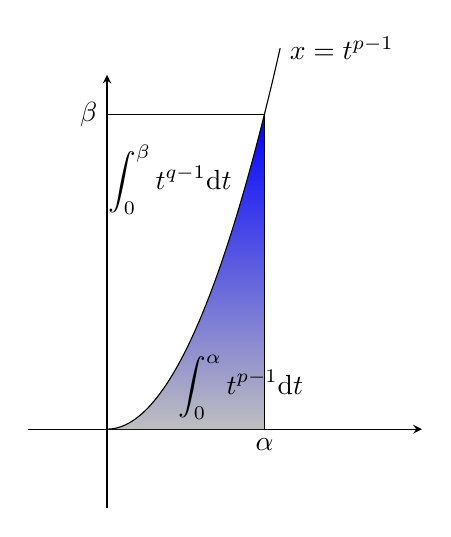
\begin{tikzpicture}[>=stealth]
\draw[->](-1,0)--(4,0);
\draw[->](0,-1)--(0,4.5);
\shade[top color=blue, bottom color=gray!50,domain=0:2,scale=1](0,0)plot({\x},{\x*\x})|-(0,0);
\draw(0,4)--(2,4)--(2,0);
\draw (2,0)node[below]{$\alpha$}
(0,4)node[left]{$\beta$};
\draw(1.7,0)node[above]{$\displaystyle{\int^{\alpha}_0t^{p-1}\mathrm{d}t}$};
\draw(0.8,2.6)node[above]{$\displaystyle{\int^{\beta}_0t^{q-1}\mathrm{d}t}$};
\draw[domain=0:2.2,smooth, variable=\x]plot({\x},{\x*\x})node[right]{$x= t^{p-1}$};
\end{tikzpicture}
\end{figure}


$$\alpha \beta \leq \frac{\alpha^p}{p}+\frac{\beta^q}{q}$$


\end{proof}

\begin{thm}[H\"older's inequality]

If $p,q>1$ and $\dfrac{1}{p}+\dfrac{1}{q}=1$, and let $\{x_i\}$ and $\{y_i\}$ be infinite sequences of complex numbers satisfying $\sum\limits^{\infty}_{i=1}|x_i|^p<\infty$ and $\sum\limits^{\infty}_{i=1}|y_i|^q<\infty$, then \begin{equation}\sum^{\infty}_{i=1}|x_iy_i|\leq \Bigg[\sum^{\infty}_{i=1}|x_i|^p\Bigg]^{\frac{1}{p}}\Bigg[\sum^{\infty}_{i=1}|y_i|^q\Bigg]^{\frac{1}{q}}\tag{2}\end{equation}


\end{thm}

\begin{proof}

Set $\hspace{0.3cm} \displaystyle{x'_i=\frac{x_i}{\Bigg[\sum\limits^{\infty}_{i=1}|x_i|^p\Bigg]^{\frac{1}{p}}}}\hspace{0.3cm}$ and $\hspace{0.3cm} \displaystyle{y'_i=\frac{y_i}{\Bigg[\sum\limits^{\infty}_{i=1}|y_i|^q\Bigg]^{\frac{1}{q}}}}$

 
Now $\hspace{0.5cm}\displaystyle{|x'_i|=\frac{|x_i|}{\Bigg[\sum\limits^{\infty}_{i=1}|x_i|^p\Bigg]^{\frac{1}{p}}}\hspace{1cm},\hspace{1cm} |y'_i|=\frac{|y_i|}{\Bigg[\sum\limits^{\infty}_{i=1}|y_i|^q\Bigg]^{\frac{1}{q}}}}$

 
$$\implies |x'_i|^p=\frac{|x_i|^p}{\sum\limits^{\infty}_{i=1}|x_i|^p}\hspace{1cm},\hspace{1cm} |y'_i|^q =\frac{|y_i|^q}{\sum\limits^{\infty}_{i=1}|y_i|^q}$$\\ $$\implies \sum^{\infty}_{i=1}|x'_i|^p=\frac{\sum\limits^{\infty}_{i=1}|x_i|^p}{\sum\limits^{\infty}_{i=1}|x_i|^p}=1\hspace{1cm},\hspace{1cm}\sum^{\infty}_{i=1}|y'_i|^q=\frac{\sum\limits^{\infty}_{i=1}|y_i|^q}{\sum\limits^{\infty}_{i=1}|y_i|^q}=1$$ Now, using the inequality $(1)$ in $(2)$, we have for any $i$ $$|x'_i||y'_i|=|x'_iy'_i|\leq \frac{|x'_i|^p}{p}+\frac{|y'_i|^q}{q}$$ Therefore,
\begin{align*}
\sum_{i=1}^{\infty}|x'_iy'_i| &\leq \frac{\sum\limits^{\infty}_{i=1}|x'_i|^p}{p}+\frac{\sum\limits^{\infty}_{i=1}|y'_i|^q}{q}
                              =\frac{1}{p}+\frac{1}{q}
                              =1
\end{align*}
$$\implies \sum^{\infty}_{i=1}|x'_iy'_i|\leq 1\implies \sum^{\infty}_{i=1}|x'_i||y'_i|\leq 1$$\\ $$\implies \sum_{i=1}^{\infty}\Bigg\{\frac{|x_i|}{\Big[\sum\limits^{\infty}_{i=1}|x_i|^p\Big]^{\frac{1}{p}}}\Bigg\} \Bigg\{\frac{|y_i|}{\Big[\sum\limits^{\infty}_{i=1}|y_i|^q\Big]^{\frac{1}{q}}}\Bigg\} \leq 1$$\\ Hence we have,$$\sum^{\infty}_{i=1}|x_i||y_i|=\sum^{\infty}_{i=1}|x_iy_i|\leq \Bigg[\sum^{\infty}_{i=1}|x_i|^p\Bigg]^{\frac{1}{p}}\Bigg[\sum^{\infty}_{i=1}|y_i|^q\Bigg]^{\frac{1}{q}}.$$


\end{proof}

\begin{coro}[The Cauchy--Schwarz inequality]
Let $p=2$ and $q=2$ and $x_i,y_i$ where $i=1,2,\dots,n$ be sets of complex numbers. Then $$\sum^n_{i=1}|x_iy_i|\leq \Bigg[\sum^n_{i=1}|x_i|^2\Bigg]^{\frac{1}{2}} \Bigg[\sum^n_{i=1}|y_i|^2\Bigg]^{\frac{1}{2}}$$ (It has the same form even for infinity sequences )

\end{coro}

\begin{proof}
Take $p=q=2$ in H\"older's inequality, which is legitimate since
$\frac12+\frac12=1$. The exponents $\frac1p$ and $\frac1q$ both become
$\frac12$, and the two bracketed sums become square roots, giving the stated
form at once.
\end{proof}

\begin{remark}[Integral form of H\"older's inequality]
Let $x=x(t)$ and $y=y(t)$ be two complex functions defined on $[0,1]$ satisfying $\displaystyle{\int^1_0|x(t)|^pdt<\infty}$ and $\displaystyle{\int^1_0|y(t)|^qdt<\infty}$. If $p,q>1$ and $\dfrac{1}{p}+\dfrac{1}{q}=1$, then $$\int^1_0|x(t)y(t)|dt\leq \Bigg[\int^1_0|x(t)|^pdt\Bigg]^{\frac{1}{p}}\Bigg[\int^1_0|y(t)|^qdt\Bigg]^{\frac{1}{q}}$$


\end{remark}

\begin{thm}[Minkowski's inequality]
If $p\geq 1$ and $(x_i)$ and $(y_i)$ are two sequences of complex numbers such that $\sum\limits^{\infty}_{i=1}|x_i|^p<\infty$ and $\sum\limits^{\infty}_{i=1}|y_i|^p<\infty$, then $$\Bigg[\sum^{\infty}_{i=1}|x_i+y_i|^p\Bigg]^{\frac{1}{p}}\leq \Bigg[\sum^{\infty}_{i=1}|x_i|^p\Bigg]^{\frac{1}{p}}+\Bigg[\sum^{\infty}_{i=1}|y_i|^p\Bigg]^{\frac{1}{p}}.$$

\end{thm}

\begin{proof}
If $p=1$, this is obvious.

Let $p>1$, write $\hspace{0.3cm}\displaystyle{|x_i+y_i|^p=|x_i+y_i||x_i+y_i|^{p-1}}$.\hspace{0.3cm} Thus,
\begin{align*}
|x_i+y_i|^p &=|x_i+y_i||x_i+y_i|^{p-1}\\
            &\leq \Big[|x_i|+|y_i|\Big]|x_i+y_i|^{p-1}\\
            &=|x_i||x_i+y_i|^{p-1}+|y_i||x_i+y_i|^{p-1}
\end{align*}
Now, consider $\hspace{0.3cm}\displaystyle{\sum^{\infty}_{i=1}|x_i||x_i+y_i|^{p-1}}\hspace{0.3cm},$ if $q$ is the conjugate of $p$\hspace{0.2cm} i.e $\hspace{0.3cm}\dfrac{1}{p}+\dfrac{1}{q}=1$.
Then
\begin{align*}
\sum^{\infty}_{i=1}|x_i||x_i+y_i|^{p-1} &\leq \Bigg[\sum^{\infty}_{i=1}|x_i|^p\Bigg]^{\frac{1}{p}} \Bigg[\sum^{\infty}_{i=1}\Big(|x_i+y_i|^{p-1}\Big)^q\Bigg]^{\frac{1}{q}}\\
                                        &=\Bigg[\sum^{\infty}_{i=1}|x_i|^p\Bigg]^{\frac{1}{p}}\Bigg[\sum^{\infty}_{i=1}|x_i+y_i|^p\Bigg]^{\frac{1}{q}}
\end{align*}
Therefore, $$\sum^{\infty}_{i=1}|x_i||x_i+y_i|^{p-1}\leq \Bigg[\sum^{\infty}_{i=1}|x_i|^p\Bigg]^{\frac{1}{p}}\Bigg[\sum^{\infty}_{i=1}|x_i+y_i|^p\Bigg]^{\frac{1}{q}}\qquad (*)$$ Similarly, $$\sum^{\infty}_{i=1}|y_i||x_i+y_i|^{p-1}\leq \Bigg[\sum^{\infty}_{i=1}|y_i|^p\Bigg]^{\frac{1}{p}}\Bigg[\sum^{\infty}_{i=1}|x_i+y_i|^p\Bigg]^{\frac{1}{q}}\dots(**)$$ Hence using $(*)$ and $(**)$, we get $$\sum^{\infty}_{i=1}|x_i+y_i|^p\leq \Bigg[\sum^{\infty}_{i=1}|x_i|^p\Bigg]^{\frac{1}{p}}\Bigg[\sum^{\infty}_{i=1}|x_i+y_i|^p\Bigg]^{\frac{1}{q}}+\Bigg[\sum^{\infty}_{i=1}|y_i|^p\Bigg]^{\frac{1}{p}}\Bigg[\sum^{\infty}_{i=1}|x_i+y_i|^p\Bigg]^{\frac{1}{q}}$$

divide both sides by $\hspace{0.3cm}\displaystyle{\Bigg[\sum^{\infty}_{i=1}|x_i+y_i|^p\Bigg]^{\frac{1}{q}}}.\hspace{0.3cm}$ We get $$\Bigg[\sum^{\infty}_{i=1}|x_i+y_i|^p\Bigg]^{\frac{1}{p}}\leq \Bigg[\sum^{\infty}_{i=1}|x_i|^p\Bigg]^{\frac{1}{p}}+\Bigg[\sum^{\infty}_{i=1}|y_i|^p\Bigg]^{\frac{1}{p}}.$$\\
(It also has the integral form)

\end{proof}


\begin{defn}
Let $X$ be a vector space, we define a norm on $X$ as a map from $X$ to $\mathbb{F}$ a vector field satisfying the following properties for all $x,y\in X$ and $\alpha \in \mathbb{F}$:
\begin{enumerate}
\item[i] $||x||\geq 0$, $||x||=0$ iff $x=0$
\item[ii] $||\alpha x||=|\alpha|||x||$, where $\alpha$ is a scalar
\item[iii] $||x+y||\leq ||x|| +||y||$.
\end{enumerate}
\end{defn}


\begin{exa}
Let $X=\mathbb{R}^n$, define $||.||$ on $\mathbb{R}^n$ by $\hspace{0.3cm}\displaystyle{||x||=\Bigg[\sum^{n}_{i=1}|x_i|^2\Bigg]^{\frac{1}{2}}}$

\end{exa}


\textbf{Check}
\begin{enumerate}
\item[i] $\hspace{0.4cm}\displaystyle{||x||=\Bigg[\sum^{n}_{i=1}|x_i|^2\Bigg]^{\frac{1}{2}}\geq 0},$\\ $$|x_i|^2=0\implies x_i=0\iff x=(0,0,\dots0)=0$$\\

\item[ii]
\begin{align*}
||\alpha x|| &=\Bigg[\sum^n_{i=1}|\alpha x_i|^2\Bigg]^{\frac{1}{2}}
              =\Bigg[\sum^n_{i=1}|\alpha|^2|x_i|^2\Bigg]^{\frac{1}{2}}\\
             &=|\alpha|\Bigg[\sum^n_{i=1}|x_i|^2\Bigg]^{\frac{1}{2}}\\
             &=|\alpha|||x||\\
\end{align*}
\item[iii]
\begin{align*}
||x+y|| &=\Bigg[\sum^n_{i=1}|x_i+y_i|^2\Bigg]^{\frac{1}{2}}\\
        &\leq \Bigg[\sum^n_{i=1}|x_i|^2\Bigg]^{\frac{1}{2}}+\Bigg[\sum^n_{i=1}|y_i|^2\Bigg]^{\frac{1}{2}}\\
        &=||x||+||y||\\
\end{align*}
\end{enumerate}
Now consider $l_p$, the space of complex sequences $x=\{x_n\}=\{x_1,x_2,\dots,\}$ such that $\sum\limits^{\infty}_{i=1}|x_i|^p<\infty$. Define a norm on $l_p$ by $$||x||=\Bigg[\sum^{\infty}_{i=1}|x_i|^p\Bigg]^{\frac{1}{p}}$$\\

We shall discuss in detail on norms in chapter 4.

\pagebreak


\section{Compact Metric Spaces}
A metric is the least structure on which a limit can be defined: a rule giving
the distance between two points, subject to four requirements. Everything in
this section is an attempt to say which metric spaces behave like closed
bounded intervals of $\mathbb{R}$.

The section develops the vocabulary first --- open and closed sets, limits and
limit points, dense and nowhere dense sets, separability --- and then the three
descriptions of compactness: every open cover has a finite subcover, every
sequence has a convergent subsequence, and totally bounded together with
complete. That these agree is the Heine--Borel theorem.

The pay-off is at the end. On a compact space a continuous function is
automatically uniformly continuous and attains its bounds, which are exactly the
facts that make the fixed point argument of Section~3 work.

\begin{defn}
Let $X$ be a non-empty set, a mapping $d:X\times X\rightarrow \mathbb{R}$ which satisfies the following for all $x,y,z\in X$:
\begin{enumerate}
\item[i] $d(x,y)\geq 0$
\item[ii] $d(x,y)=0$ if and only if $x=y$
\item[iii] $d(x,y)=d(y,x)$
\item[iv] $d(x,z)\leq d(x,y)+d(y,z)$ (triangle inequality)
\end{enumerate}
The pair $(X,d)$ is called a metric space.

\end{defn}


\begin{exa}
The function $d(x,y)=|x-y|$ defines a metric on $\mathbb{R}$. This is called the usual metric on $\mathbb{R}$.


\textbf{Proof} By definition, the absolute value on $\mathbb{R}$ is non-negative. Therefore  $\hspace{0.3cm} d(x,y)=|x-y|\geq 0$.

Now, since $|x-y|=0$ if and only if $x=y$. It follows that $d(x,y)=0$ if and only if $x=y$.

To verify the third axiom, we have $\hspace{0.3cm} d(x,y)=|x-y|=|-(y-x)|=|y-x|=d(y,x)$.\\To verify the triangle inequality, suppose that $x,y,z\in \mathbb{R}$ then 
\begin{align*}
d(x,z) &=|x-z|=|x-y+y-z|\\
       &\leq |x-y|+|y-z|\\
       &=d(x,y)+d(y,z)
\end{align*} 
Hence $(\mathbb{R},d)$ is a metric space.

\end{exa}


\begin{exa}
$\mathbb{C}$, the set of complex numbers with the function $d(u,v)=|u-v|$ for $u,v\in \mathbb{C}$.

\end{exa}
\begin{proof}
\begin{enumerate}
\item[i] 
\begin{align*}
d(u,v) &=|(u_1+iu_2)-(v_1+iv_2)|
       =|(u_1-v_1)+i(u_2-v_2)|\\
       &=\sqrt{(u_1-v_1)^2+(u_2-v_2)^2}\geq 0
\end{align*}
\item[ii] $\hspace{0.2cm} d(u,v)=|u-v|=0\iff u_1-v_1=0, u_2-v_2=0\implies u_1=v_1,u_2=v_2\implies u=v$
\item[iii]
\begin{align*}
d(u,v) &=|(u_1+iu_2)-(v_1+iv_2)|
        =|-((v_1+iv_2)-(u_1+iu_2))|\\
       &=|(v_1+iv_2)-(u_1+iu_2)|\\
       &=d(v,u)
\end{align*}
\item[iv] Let $u,v,w\in \mathbb{C}$,then
\begin{align*}
d(u,w) &=|(u_1+iu_2)-(w_1+iw_2)|\\
       &=|(u_1+iu_2)-(v_1+iv_2)+(v_1+iv_2)-(w_1+iw_2)|\\
       &\leq |(u_1+iu_2)-(v_1+iv_2)|+|(v_1+iv_2)-(w_1+iw_2)|\\
       &=d(u,v)+d(v,w)
\end{align*}
\end{enumerate}
Hence $(\mathbb{C},d)$ is a metric space.

\end{proof}


\begin{exa}
If $x=(x_1,x_2),y=(y_1,y_2)$ in $\mathbb{R}^2$ we define $d:\mathbb{R}^2\times \mathbb{R}^2\rightarrow \mathbb{R}$ by $$d(x,y)=\max\{|x_1-y_1|,|x_2-y_2|\}$$
\end{exa}
\begin{proof}
If $x=(x_1,x_2),y=(y_1,y_2)\in \mathbb{R}^2$, we see that $|x_1-y_1|\geq 0$ and $|x_2-y_2|\geq 0$ so that $$d(x,y)=\max\{|x_1-y_1|,|x_2-y_2|\}\geq 0.$$
Also, $\max\{|x_1-y_1|,|x_2-y_2|\}=0$ if and only if $|x_1-y_1|=0$ and $|x_2-y_2|=0$, which means that $\max\{|x_1-y_1|,|x_2-y_2|\}=0$ if and only if $x_1=y_1$ and $x_2=y_2$. Thus $d(x,y)=0$ if and only if $x=y$.

We show that $d(x,y)=d(y,x)$. Since $\max\{|x_1-y_1|,|x_2-y_2|\}=\max\{|y_1-x_1|,|y_2-x_2|\}$, we have that $d(x,y)=d(y,x)$.

To show the triangle inequality holds, let $x=(x_1,x_2), y=(y_1,y_2), z=(z_1,z_2)\in \mathbb{R}^2$. Then
\begin{align*}
d(x,z) &=\max\{|x_1-z_1|,|x_2-z_2|\}\\
       &=\max\{|x_1-y_1+y_1-z_1|,|x_2-y_2+y_2-z_2|\}\\
       &\leq \max\{|x_1-y_1|+|y_1-z_1|,|x_2-y_2|+|y_2-z_2|\}\\
       &\leq \max\{|x_1-y_1|,|x_2-y_2|\}+\max\{|y_1-z_1|,|y_2-z_2|\}\\
       &=d(x,y)+d(y,z).
\end{align*}
Hence $(\mathbb{R}^2,d)$ is a metric space.

\end{proof}


\begin{exa}
Let $x=(x_1,x_2)$, $y=(y_1,y_2)\in \mathbb{R}^2$ and define
$d:\mathbb{R}^2\times \mathbb{R}^2\rightarrow \mathbb{R}$ by
$$d(x,y)=|x_1-y_1|+|x_2-y_2| .$$
Check whether $(\mathbb{R}^2,d)$ is a metric space.
\end{exa}
\begin{solution}
All four axioms must be checked. Write $z=(z_1,z_2)$ for a third point.

\subhead{Non-negativity}
Each term is an absolute value, so $d(x,y)\geq 0$ always.

\subhead{$d(x,y)=0$ if and only if $x=y$}
A sum of two non-negative numbers is zero only if both are, so $d(x,y)=0$
forces $|x_1-y_1|=0$ and $|x_2-y_2|=0$, that is $x_1=y_1$ and $x_2=y_2$, which
is $x=y$. Conversely $d(x,x)=0+0=0$.

\subhead{Symmetry}
$|a-b|=|b-a|$ for real $a,b$, so
$$d(x,y)=|x_1-y_1|+|x_2-y_2|=|y_1-x_1|+|y_2-x_2|=d(y,x).$$

\subhead{Triangle inequality}
Apply the triangle inequality for real numbers to each coordinate:
$$|x_i-z_i|\leq |x_i-y_i|+|y_i-z_i|,\qquad i=1,2 .$$
Adding the two,
$$d(x,z)=\sum_{i=1}^{2}|x_i-z_i|
\leq \sum_{i=1}^{2}|x_i-y_i|+\sum_{i=1}^{2}|y_i-z_i|=d(x,y)+d(y,z).$$

All four hold, so $(\mathbb{R}^2,d)$ \emph{is} a metric space. This $d$ is the
\emph{taxicab} metric: it measures distance as a car would travel on a square
grid, and it is genuinely different from the Euclidean metric --- the points at
distance $1$ from the origin form a diamond, not a circle.
\end{solution}


\begin{proof}
\begin{enumerate}
\item[i] $d(x,y)=|x_1-y_1|+|x_2-y_2|\geq 0$ since $|x_1-y_1|\geq 0$ and $|x_2-y_2|\geq 0$.
\item[ii] $d(x,y)=|x_1-y_1|+|x_2-y_2|=0\iff x_1-y_1=0, x_2-y_2=0\\ \implies x_1=y_1, x_2=y_2\implies x=y$.
\item[iii] $\hspace{0.2cm} d(x,y)=|x_1-y_1+|x_2-y_2|=|-(y_1-x_1)|+|-(y_2-x_2)|=|y_1-x_1|+|y_2-x_2|=d(y,x)$
\item[iv] 
\begin{align*}
d(x,z) &=|x_1-z_1|+|x_2-z_2|\\
       &=|x_1-y_1+y_1-z_1|+|x_2-y_2+y_2-z_2|\\
       &\leq |x_1-y_1|+|y_1-z_1|+|x_2-y_2|+|y_2-z_2|\\
       &=(|x_1-y_1|+|x_2-y_2|)+(|y_1-z_1|+|y_2-z_2|)\\
       &=d(x,y)+d(y,z)
\end{align*}
$\implies d(x,z)\leq d(x,y)+d(y,z)$ Hence $(\mathbb{R}^2,d)$ is a metric space.
\end{enumerate}
\end{proof}

\begin{exa}
\begin{enumerate}
\item The set $\mathbb{R}^2$ of ordered pairs $(x_1,x_2)\in \mathbb{R}^2$. The metric defined by $$d(x,y)=\sqrt{(x_1-y_1)^2+(x_2-y_2)^2}$$ Where $x=(x_1,x_2), y=(y_1,y_2)\in \mathbb{R}^2$.  Check if $(\mathbb{R}^2,d)$ is a metric space.
\item If $x=(x_1,x_2,\dots,x_n)$, $y=(y_1,y_2,\dots,y_n)$ are two points in $\mathbb{R}^n$ define a metric as follows $d:\mathbb{R}^n\times \mathbb{R}^n\rightarrow \mathbb{R}$ as $$d(x,y)=\sqrt{(x_1-y_1)^2+(x_2-y_2)^2+\cdots+(x_n-y_n)^2}=\Bigg[\sum^n_{i=1}(x_i-y_i)^2\Bigg]^{\frac{1}{2}}$$ The space $(\mathbb{R}^n,d)$ is a metric space.
\item If $p\geq$ and $x=(x_1,x_2,\dots,x_n)$ and $y=(y_1,y_2,\dots,y_n)$ be any two elements of the space $l_p^n$, define the metric $d:l_p^n\times l_p^n\rightarrow \mathbb{R}$ as follows $$d(x,y)=\Bigg[\sum^n_{i=1}|x_i-y_i|^p\Bigg]^{\frac{1}{p}}$$ Prove that $l^n_p$ with this metric is a metric space.\\ 
\end{enumerate}


\pagebreak

\subhead{Limit of a sequence in $(X,d)$}

\begin{defn}
Let $(S_n)$ be a sequence of points in a metric space $X$. We say that $S_n\rightarrow l$ in $X$ as $n\rightarrow \infty$ if given $\varepsilon >0$, $\exists$ a positive integer $n_0$ such that $\hspace{0.3cm}\displaystyle{ d(S_n,l)<\varepsilon \hspace{0.4cm} \forall n\geq n_0}.$


Denote this as $\lim\limits_{n\rightarrow \infty}S_n=l$.


In other words, we say that $(S_n)$ has a limit and converges to $l$.

\end{defn}

\begin{exa}
\begin{enumerate}
\item Let $X=\mathbb{R}$, $\hspace{0.3cm} d(S_n,l)=|S_n-l|$
\item $X=\mathbb{C}$, $\hspace{0.3cm} d(S_n,l)=|S_n-l|$
\item Let $X=\mathbb{R}^n$, $\hspace{0.4cm}\displaystyle{ d(S_n,l)=\Bigg[\sum^n_{i=1}|S_n-l|^2\Bigg]^{\frac{1}{2}}}$
\item $X=l_{\infty}$ space of bounded sequences, $\hspace{0.3cm}\displaystyle{ d(S_n,l)=\sup_{1\leq n<\infty}|S_n-l|}.$
\end{enumerate}
\end{exa}


\begin{defn}
Let $(X,d)$ be a metric space and $(S_n)$ be a sequence of points in $X$. We say that $(S_n)$ is a Cauchy sequence in $X$ if given $\varepsilon >0$, $\exists$ a natural number $n_0$ such that $\hspace{0.2cm}\displaystyle{ d(S_m,S_n)<\varepsilon \hspace{0.4cm} \forall m,n\geq n_0}$


In other words, $d(S_m,S_n)\rightarrow 0$ as $m,n\rightarrow \infty$.

\end{defn}


\begin{exa}
Let $X=\mathbb{R}\,$ and $\hspace{0.3cm}\displaystyle{ S_n=1-\frac{1}{2}+\frac{1}{3}-\frac{1}{4}+\cdots+\frac{(-1)^{n-1}}{n}}\hspace{0.3cm}$ Is $(S_n)$ a Cauchy sequence?

\end{exa}

\begin{solution}
Let $m>n\geq n_0$ we have 
\begin{align*}
|S_m-S_n| &=\Big|\frac{(-1)^{n}}{n+1}+\cdots+\frac{(-1)^{m-1}}{m}\Big|\\
          &=\Big|\frac{1}{n+1}-\frac{1}{(n+2)(n+3)}-\frac{1}{(n+4)(n+5)}-\cdots-\Big|
\end{align*}
with negative last term $\hspace{0.3cm}\dfrac{1}{m}<\dfrac{1}{n}<\dfrac{1}{n_0}\hspace{0.2cm},\hspace{0.3cm}$ choose $n_0>\frac{1}{\varepsilon}$ then $|S_m-S_n|<\varepsilon$ whenever $n_0>\dfrac{1}{\varepsilon}$ so $(S_n)$ is Cauchy in $\mathbb{R}$.

\end{solution}


\begin{thm}
A convergent sequence in a metric space $(X,d)$ has a unique limit in $X$.
\end{thm}
\begin{proof}
Suppose $(S_n)$ converges to both $l$ and $l'$. The strategy is to show
$d(l,l')$ is smaller than every positive number, which for a metric leaves only
one possibility.

Let $\varepsilon>0$. By convergence to $l$ there is $N_1$ with
$d(S_n,l)<\frac{\varepsilon}{2}$ for $n\geq N_1$, and by convergence to $l'$
there is $N_2$ with $d(S_n,l')<\frac{\varepsilon}{2}$ for $n\geq N_2$. Take
$n\geq\max(N_1,N_2)$; then by the triangle inequality
$$0\leq d(l,l')\leq d(l,S_n)+d(S_n,l')<\frac{\varepsilon}{2}+\frac{\varepsilon}{2}
=\varepsilon .$$
So $0\leq d(l,l')<\varepsilon$ for every $\varepsilon>0$, which forces
$d(l,l')=0$, and by the second metric axiom $l=l'$.

Note where the axioms are used: the triangle inequality to compare the two
limits through a common term, and $d(x,y)=0\Rightarrow x=y$ to convert distance
zero into equality. Without the second axiom the limit need not be unique,
which is exactly what happens in a pseudometric space.
\end{proof}


\begin{proof}
Let $(S_n)$ be a convergent sequence in $(X,d)$. If the limit is not unique, then it may be $l_1$ or $l_2$. This means that $$d(S_n,l_1)<\frac{\varepsilon}{2}\hspace{0.5cm}\forall n\geq n_1$$ $$d(S_n,l_2)<\frac{\varepsilon}{2}\hspace{0.5cm} \forall n\geq n_2$$ Take $n_0=\max\{n_1,n_2\}$, then we have $$0\leq d(l_1,l_2)\leq d(S_n,l_1)+d(S_n,l_2)<\frac{\varepsilon}{2}+\frac{\varepsilon}{2}=\varepsilon \hspace{0.3cm} \forall n\geq n_0$$ $d(l_1,l_2)\rightarrow 0$ as $n\rightarrow \infty$. Thus $l_1$ and $l_2$ are but the same.
\end{proof}


\begin{thm}
Every convergent sequence in $(X,d)$ is a Cauchy sequence in $(X,d)$.

\end{thm}

\begin{proof}
Let $(S_n)$ be a convergent sequence in $(X,d)$. i.e $\lim\limits_{n\rightarrow \infty}S_n=l$ where $l\in (X,d)$. Then $$0\leq d(S_n,S_m)\leq d(S_n,l)+d(S_m,l)\rightarrow 0\hspace{0.3cm}\text{as}\hspace{0.3cm} n,m\rightarrow \infty.$$ Hence $(S_n)$ is Cauchy.\\\\
\textbf{Note:} The converse of this statement is not true in general.

\end{proof}
In order to see this, we consider a counter example.

\end{exa}
\begin{exa}
Let $E=(0,1)\subset \mathbb{R}$. Take $S_n=\frac{1}{n}$ in $E$.\\ Note that $(S_n)$ is a Cauchy sequence in $E$. $$0\leq d(S_n,S_m)=\Big|\frac{1}{n}-\frac{1}{m}\Big|\leq \dfrac{1}{n}+\frac{1}{m}\rightarrow 0\hspace{0.3cm}\text{as}\hspace{0.3cm} n,m\rightarrow \infty.$$ 
But $\lim\limits_{n\rightarrow \infty}S_n=\lim\limits_{n\rightarrow \infty}\dfrac{1}{n}=0\not\in E$. In other words, no point of $E=(0,1)$ can be a limit of the sequence $(S_n)=\dfrac{1}{n}$.


\pagebreak

\subhead{Bounded Sets}

\begin{defn}
A subset $E$ of $(X,d)$ is said to be bounded if $\exists$ a positive real number $M$ such that $$d(x,y)\leq M\hspace{0.5cm} \forall x,y\in E.$$

If $A$ is bounded, then $\dim(A)<\infty$, where $\hspace{0.2cm}\dim(A)=\sup \{d(x,y), x,y\in A\}$


If $\dim(A)=\infty$, the set $A$ is unbounded.

\end{defn}


\begin{exa}
Any finite set in a metric space is bounded.

\end{exa}


\begin{thm}
Every Cauchy sequence in a metric space is bounded.

\end{thm}
\end{exa}

\begin{proof}
Let $(x_n)$ be Cauchy in $(X,d)$, this means $d(x_n,x_m)<\varepsilon$ for all $n,m\geq n_0$. Now, take $\varepsilon =1$. Take $\hspace{0.2cm}\displaystyle{ M=\max_{1\leq n\leq n_0}\{d(x_n,x_{n_0})\}<\infty}.\hspace{0.2cm}$ Now $\hspace{0.2cm} \displaystyle{d(x_n,x_m)\leq d(x_n,x_{n_0})+d(x_{n_0},x_m)}.\hspace{0.2cm}$ Now, $$d(x_n,x_{n_0})<M+1\hspace{0.5cm} \forall n$$ $$d(x_{n_0},x_m)<M+1\hspace{0.5cm} \forall n$$ Therefore, $\hspace{0.2cm} \displaystyle{d(x_n,x_m)\leq d(x_n,x_{n_0})+d(x_{n_0},x_m)<2(M+1)\hspace{0.3cm} \forall m,n\geq n_0}.\hspace{0.2cm}$ Let $K=2(M+1)$, we have that $\hspace{0.2cm} \displaystyle{d(x_n,x_m)\leq K,\hspace{0.5cm} \forall n,m}.\hspace{0.2cm}$ Thus every Cauchy sequence is bounded in $(X,d)$.\\\\


\pagebreak
\subhead{Limit and Continuity of a function in $(X,d)$}

\begin{defn}
Let $(X,d_X)$ and $(Y,d_Y)$ be metric spaces and $x_0\in X$. The function $f:X\rightarrow Y$ is said to approach a limit $l\in Y$ as $x$ approaches $x_0$ if given $\varepsilon >0, \exists \delta >0\ni d_Y(f(x),l)<\varepsilon$ whenever $0<d_X(x,x_0)<\delta$.

\end{defn}


\begin{defn}
Let $(X,d_X)$ and $(Y,d_Y)$ be metric spaces. Let $f:X\rightarrow Y$ be a function. The function $f$ is said to be continuous at $x_0\in X$ if given $\varepsilon >0,\exists \delta >0\ni d_Y(f(x),f(x_0))<\varepsilon$ whenever $d_X(x,x_0)<\delta$.

\end{defn}


\begin{defn}
Let $(X,d)$ be a metric space, if $x_0\in X$ and $r>0$, then the open ball or (open sphere) is the set $B_r(x_0)=\{x\in X:d(x,x_0)<r\}$ or $S_r(x_0)=\{x\in X:d(x,x_0)<r\}.$

\end{defn}


\begin{exa}
Let $X=\mathbb{R}$ with the usual metric, then $B_r(x_0)=\{x\in \mathbb{R}:|x-x_0|<r\}$ or as an interval $(x_0-r,x_0+r)$.

\end{exa}

\begin{thm}
Let $(X,d_X)$ and $(Y,d_Y)$ be metric spaces and let $f:X\rightarrow Y$ be a function, then $f$ is continuous if and only if $f^{-1}(G)$ is an open set in $X$ whenever $G$ is an open set in $Y$.

\end{thm}

\begin{proof}
Let $f$ be continuous and $G$ be an open set in $Y$. Then to prove that $f^{-1}(G)$ is open in $X$. Choose an arbitrary point $x\in f^{-1}(G)$, then $f(x)\in G$. Now, since $G$ is open in $Y$, it follows that $B_r(f(x))\subseteq G\qquad (1)$. Since $f$ is continuous , it follows that\\ $f(B_{\delta}(x))\subseteq B_r(f(x))\qquad (2).\hspace{0.2cm}$ Using $(1)$ and $(2)$ to get $$f(B_{\delta}(x))\subseteq G$$ $$B_{\delta}(x)\subseteq f^{-1}(G)$$ Thus we've found an open ball for any $x\in f^{-1}(G)$. Thus $f^{-1}(G)$ is open in $X$.\\ 
Conversely, Let $G$ be an open set in $Y$ and $f^{-1}(G)$ be also open. Then to prove that $f$ is continuous. Consider the open set $G=B_r(f(x))$. Then $\exists$ some $\delta >0\ni B_{\delta}(x)\subseteq f^{-1}(G)$. Therefore $\hspace{0.2cm} f(B_{\delta}(x))\subseteq G=B_r(f(x)).\hspace{0.2cm}$ This shows continuity.

\end{proof}


\begin{defn}
Let $(X,d_X)$ and $(Y,d_Y)$ be metric spaces and let $f:X\rightarrow Y$. We say that $f$ is uniformly continuous if for every $\varepsilon >0, \exists \delta >0\ni d_Y(f(x_1),f(x_2))<\varepsilon$ whenever $d_X(x_1,x_2)<\delta$ where $x_1,x_2\in X$.

\end{defn}
\end{proof}


\textbf{Countable Sets}

. Two sets $A$ and $B$ are equivalent if there exists one-one correspondence between $A$ and $B$.

. Every set $A$ is equivalent to itself.

. If $A$ and $B$ are equivalent then $B$ and $A$ are equivalent. ($\exists$ a bijection)


E.g $\mathbb{N}$ is equivalent to a proper subset of itself like 2,4,8,16,\dots where the one-one map is $f:X\rightarrow 2^x$.


\textbf{Finite Set}

A subset $A$ is finite if it is empty or if $\exists$ a natural number $n$ such that $A$ is equivalent to $\{1,2,3,\dots,n\}$.


\textbf{Infinite Set}

A set $A$ is infinite if it not finite.


\begin{defn}
A set $A$ is said to be countable if $A$ is finite or equivalent to the set of all positive integers.


i.e $\exists$ one-one from $\mathbb{N}$ to $A$. The elements of $A$ are the images of the positive integers.

\end{defn}


\begin{exa}
$E$ the set of even natural numbers is countable. The function $f(n)=2n$ for each $n\in \mathbb{N}$ gives a one-one correspondence.

\end{exa}


\begin{exa}
The set $\mathbb{Z}$ of integers is countable. Define a function $f:\mathbb{N}\rightarrow \mathbb{Z}$
\[f(n)=
\begin{cases}
\dfrac{n-1}{2}, &n=1,3,5,\dots\\
\dfrac{-n}{2},  &n=2,4,6\dots
\end{cases}
\]

Find another function $h:\mathbb{N}\rightarrow \mathbb{Z}$.

\end{exa}


\begin{thm}
Every infinite set has a countable subset.

\end{thm}


\begin{thm}
Every infinite set is equivalent to one of its proper subsets.

\end{thm}


\begin{thm}
If $A_1,A_2,A_3,\dots$ are countable sets then $\bigcup\limits^{\infty}_{n=1}A_n$ is countable.

\end{thm}


\begin{coro}
The set of all rational numbers $\mathbb{Q}$ is countable.

\end{coro}


\begin{thm}
Any infinite subset of a countable set is countable.

\end{thm}


\begin{defn}
We say that  a set $E$ is uncountable if $E$ is neither finite nor countable.

\end{defn}


\begin{exa}
\begin{enumerate}
\item[a] The interval $[0,1]$ is uncountable.
\item[b] The set of all real numbers $\mathbb{R}$ is uncountable.
\item[c] The set of all irrational numbers is uncountable.
\item[d] $(0,1)$ is uncountable.
\end{enumerate}
\end{exa}


\textbf{CANTOR'S uncountable set}

To construct the Cantor set, we proceed as follows:\\ First denote the closed interval $[0,1]$ by $F_1$. Next, from $F_1$ delete the open interval $(\frac{1}{3},\frac{2}{3})$. Denote the remaining closed set by $F_2=[0,\frac{1}{3}]\cup [\frac{2}{3},1]$.\\ Next delete from $F_2$, the open interval $(\frac{1}{9},\frac{2}{9})$ and $(\frac{7}{9},\frac{8}{9})$ which are middle thirds of $F_2's$ two pieces. Denote the remaining by $$F_3=\Big[0,\frac{1}{9}\Big]\cup \Big[\frac{2}{9},\frac{1}{3}\Big]\cup \Big[\frac{2}{3},\frac{7}{9}\Big]\cup \Big[\frac{8}{9},1\Big]$$ Continuing this process, we get a sequences of $F_n$. Define the Cantor set as $$F=\bigcap^{\infty}_{i=1}F_i=F_1\cap F_2\cap F_3\cap\dots$$ $F$ is closed, since it is an intersection of closed sets.\\\\

$F$ clearly contains the end points of the closed intervals which make up each $F_n$. i.e the points $0,1,\dfrac{1}{3},\dfrac{2}{3},\dfrac{1}{9},\dfrac{2}{9},\dfrac{7}{9},\dfrac{8}{9},\dots$.

Question: Does $F$ contain any other other points?

- Observe that 1/4 is in $F$ but it is not an end point of any of the closed intervals for the $F_n's$.

- Can you find more?

$(*)$ Prove that the sum of lengths of the intervals removed from $[0,1]$ equal $1$.


\pagebreak

\textbf{Partially Ordered Sets}

Let $P$ be a non-empty set. A partial order relation in $P$ is a relation symbolized $\leq$ with the following properties for $x,y,z\in P$:
\begin{enumerate}
\item[i] $x\leq x$ (reflexive)
\item[ii] $x\leq y$ and $y\leq x\implies x=y$ (symmetric)
\item[iii] $x\leq y$  and $y\leq z\implies x\leq z$ (transitivity)
\end{enumerate}   

\begin{defn}
A non-empty set $P$ in which there is a partial order relation is called a partially ordered set,(sometimes called Poset).

Observe that any non-empty subset of a Poset is a Poset.

\end{defn}


\begin{exa}
$P$ a collection of subsets of a universal set $U$, let $A\leq B$ means that $A\subseteq B$ for all $A,B\in P$.

\end{exa}
\begin{solution}
Let $A,B,C\in P$,then 
\begin{enumerate}
\item[i] $A\leq A$, since $A\subseteq A$.
\item[ii] $A\leq B$ and $B\leq A\implies A=B$, since $A\subseteq B$ and $B\subseteq A\implies A=B$.
\item[iii] $A\leq B$ and $B\leq C\implies A\leq C$ since $A\subseteq B$ and $B\subseteq C\implies A\subseteq C$.
\end{enumerate}
\end{solution}

\begin{exa}
Let $P$ be the set of all functions defined on a non-empty set $X$. Let $f\leq g$ mean $f(x)\leq g(x)$ for every $x\in X$.

\end{exa}
\begin{solution}
\begin{enumerate}
\item[i] $f(x)\leq f(x)\hspace{0.5cm} \forall x\in X$.
\item[ii] $f(x)\leq g(x)$ and $g(x)\leq f(x)\implies f(x)=g(x)$.
\item[iii] $f(x)\leq g(x)$ and $g(x)\leq h(x)$, then $f(x)\leq h(x)$.
\end{enumerate}
\end{solution}


\begin{exa}
Let $P$ be the set $\mathbb{R}$. Let $x\leq y$ means $x$ is less or equal $y$. Then $(P,\leq)$ is a partial order relation.

\end{exa}


\textbf{Check}
\begin{enumerate}
\item[i] $x\leq x,\hspace{0.5cm} \forall x\in \mathbb{R}$.
\item[ii] $x\leq y$ and $y\leq x\implies x=y$.
\item[iii] $x\leq y$ and $y\leq z\implies x\leq z$.
\end{enumerate}

\begin{exa}
Let $P$ be the set of positive integer and let $m\leq n$ means $m$ divides $n$.

\end{exa}
\textbf{Check}

\begin{enumerate}
\item[i] $m\leq m,\hspace{0.5cm} \forall m\in \mathbb{N}$.
\item[ii] $m\leq n$ and $n\leq m\implies m=n$.
\item[iii]$m\leq n$ and $n\leq q\implies m\leq q$.
\end{enumerate}
We will look at order relations with the fourth property

iv. Any two elements are comparable.


\begin{defn}
A partial order relation with property (iv) is called a totally ordered set.
Sometimes a totally ordered set is called a chain.


\pagebreak
%COMPLETE METRIC SPACES
\end{defn}
\section{Complete Metric Spaces}
A Cauchy sequence is one whose terms eventually crowd together. In a
\emph{complete} space every such sequence actually converges, and the point of
this section is that completeness is what lets a limit be constructed before it
is known.

After establishing that $\mathbb{R}$ and $l_p$ are complete, and that a
metric space can always be completed, the section reaches the contraction
mapping theorem: a map that shrinks distances by a fixed factor has exactly one
fixed point, and the point is found by iterating from anywhere at all.

Picard's theorem is the application, and it is the reason the integral equation
on the title page is worth writing down. Recasting an initial value problem
$y'=f(t,y)$, $y(x_0)=y_0$ as
$$g(x)=y_0+\int_{x_0}^{x}f\big(t,g(t)\big)\,dt$$
turns "solve the differential equation" into "find a fixed point", and the
contraction mapping theorem then supplies existence \emph{and} uniqueness at
once.


\begin{defn}
A metric space $(X,d)$ is said to be a complete metric space if every Cauchy sequence of points in $X$ converges to some point $x\in X$.

\end{defn}


\begin{exa}
$\mathbb{R}$, the set of real numbers is a complete metric space.

\end{exa}


\begin{exa}
$\mathbb{R}^2$ is complete.

Let $x_n=(x^n_1,x^n_2)$ be a Cauchy sequence in $\mathbb{R}^2$, then given $\varepsilon >0,\exists n_0\in \mathbb{N}$,\\ $d(x_m,x_n)<\varepsilon \hspace{0.3cm} \forall m,n>n_0$. i.e $$\sqrt{(x^n_1-x_1^m)^2+(x^n_2-x^m_2)^2}<\varepsilon$$ i.e $\hspace{0.2cm}(x_1^n-x_1^m)^2+(x_2^n-x_2^m)^2<\varepsilon^2\hspace{0.3cm} m,n>n_0$
 $\implies (x_1^n-x_1^m)^2<\varepsilon^2$ and $(x_2^n-x_2^m)^2<\varepsilon^2$.

Hence we have that $x^n_1$ and $x_2^n$ are Cauchy sequences in $\mathbb{R}$. Now, every Cauchy sequence in $\mathbb{R}$ converges to some limit in $\mathbb{R}$. It means $$x_1^n\rightarrow x_1\in \mathbb{R}$$ $$x^n_2\rightarrow x_2\in \mathbb{R}$$ i.e $$|x^n_1-x_1|<\varepsilon \hspace{0.5cm} \forall n\geq n_0$$ $$|x^n_2-x_2|<\varepsilon \hspace{0.5cm} \forall n\geq n_0.$$  $$\sqrt{(x^n_1-x_1)^2+(x^n_2-x_2)^2}<\varepsilon\implies d(x_n,x)<\varepsilon \hspace{0.5cm} n\geq n_0$$ Thus $x_n$ converges to a limit $x=(x_1,x_2)\in \mathbb{R}^2$.
\end{exa}


\begin{exa}
Show that the metric space $\mathbb{R}^n$, where for $x,y\in \mathbb{R}^n$, $\hspace{0.3cm}\displaystyle{ d(x,y)=\Bigg[\sum^n_{i=1}(x_i-y_i)^2\Bigg]^{\frac{1}{2}}}$ is complete.

\end{exa}


\begin{thm}
Let $(X,d)$ be a complete metric space and let $A\subseteq X$ with some metric $d$ and $A$ is closed. Then $(A,d)$ is a complete metric space.

\end{thm}

\begin{proof}
Let $(x_n)$ be a Cauchy sequence in $(A,d)$. We need to show that $x_n\rightarrow x\in A$.

Now, since $A\subset X$, then $x_n$ is a Cauchy sequence in $X$. Thus, since $X$ is complete, $(x_n)$ must converge to a point $x\in X$. Hence $x$ is a limit point of $A$. Since $A$ is closed, we get $x\in A$. So every Cauchy sequence in $A$ converges to a point $x$ of $A$.  Hence $A$ is complete.

\end{proof}


 
\begin{exa}
$[0,1]$ is a closed subspace of $\mathbb{R}$. Now, since $\mathbb{R}$ is complete so is $[0,1]$.

\end{exa}


\begin{defn}
Let $X$ be a metric space. A subset $E$ of $X$ is said to be dense in $X$ if $\overline{E}=X$.

\end{defn}


\begin{exa}
The set $\mathbb{Q}$ of all rational numbers is dense in $\mathbb{R}$, $\hspace{0.2cm}\overline{\mathbb{Q}}=\mathbb{Q}\cup \mathbb{I}_{rr}=\mathbb{R}\hspace{0.2cm}$.  $\mathbb{Q}$ is dense in $\mathbb{R}$ because every irrational number is a limit of a sequence of rational numbers.\\ e.g$$\sqrt{2}=1.41421\dots=1+0.4+0.01+0.004+\dots$$ consider the sequence $\hspace{0.2cm}\displaystyle{\Big\{1,1+\frac{2}{5},1+\frac{2}{5}+\frac{1}{100},1+\frac{2}{5}+\frac{1}{100}+\frac{4}{1000}+\dots\Big\}}$
\end{exa}


\begin{defn}
A subset $E$ of $\mathbb{R}$ is said to be nowhere dense in $\mathbb{R}$ if $\overline{E}$ contains no non-empty open intervals.

\textbf{Note:} A closed set $E$ of $\mathbb{R}$ is nowhere dense if $E$ itself contains no open intervals.

\end{defn}


\begin{exa}
The set $\mathbb{N}$ of positive integers is nowhere dense $\hspace{0.2cm}\mathbb{N}=\{1,2,3,\dots\}\hspace{0.2cm}$ since it contains no open intervals.

\end{exa}
\begin{exa}
Let $\hspace{0.2cm}E=\Big\{1,\dfrac{1}{2},\dfrac{1}{3},\dfrac{1}{4},\dots\Big\}$ $$\overline{E}=\Big\{0,1,\frac{1}{2},\frac{1}{3},\frac{1}{4},\dots\Big\}$$ $E$ is nowhere dense because it has no  non-empty open intervals.
\end{exa}

\begin{exa}
Any one point set in $\mathbb{R}$ with the usual metric is nowhere dense.

\end{exa}

\begin{defn}
A metric space $X$ is said to be separable if there exists a countable dense subset in $X$.

\end{defn}


\begin{exa}
Let $X=\mathbb{R}$, then $X$ is separable, since $\mathbb{Q}$ is a countable and dense subset in $\mathbb{R}$.

\end{exa}


\begin{exa}
Let $X=[0,1]$ with discrete metric defined on it. Then $X$ is not a separable metric space since the only dense subset of the discrete metric space is $X$ itself.

\end{exa}


\begin{thm}
A metric space $(X,d)$ is separable if and only if $X$ has a countable subset $E$ with the following property. For every $\varepsilon>0$ and $x\in X$, there is a $y\in E$ such that $d(x,y)<\varepsilon$.

\end{thm}


\begin{proof}
Let $X$ be separable, then $X$ has a countable dense subset $E$. Let $x\in X$ and $\varepsilon>0$ be given. Since $E$ is dense in $X$, we have that $\overline{E}=X$ and $x\in \overline{E}$ so that the open ball $B_{\varepsilon}(x)$ contains a point $y\in E$. Therefore $d(x,y)<\varepsilon$.

Conversely, if $X$ has a countable subset $E$ with the given property that every $x\in X$ is a point of $E$ or limit point of $E$. Hence $\overline{E}=X$.

Therefore $X$ is separable.


A subset $A$ of a metric space $X$ is said to be dense in $X$ if $\overline{A}=X$. This is equivalent to the following:
\begin{enumerate}
\item[i] For each $x\in X$ and $\varepsilon>0$, there exists an element $a\in A\ni d(x,a)<\varepsilon$.
\item[ii] For $x\in X$, there exist $\{a_n\}\in A$ such that $a_n\rightarrow x$.(Every point $x\in X$ is a limit point of $A$).
\item[iii] Any open set in $X$ contains a point of $A$.
\end{enumerate} 
\end{proof}


\begin{exa}
Prove that the space $C_0$ is separable where $C_0=\{(x_n):x_n\rightarrow 0, n\rightarrow \infty \}$ and the metric on $C_0$ defined by $\hspace{0.2cm}\displaystyle{ d(x,y)=\sup_{1\leq n\leq \infty}|x_n-y_n|}$

\end{exa}


\begin{solution}
Let $E$ be a subset of $C_0$ consisting of all sequences of rational numbers in which only finite number of elements are different from zero. This set is a countable subset of $C_0$.

To prove that $E$ is dense in $C_0$, let $x$ be any point in $C_0$. Now, we have to find a point of $E$ whose distance from $x$ is arbitrary small. In other words, we want to select a point of $E$ whose distance from $x$ is small. That is to select a point $r=(r_1,r_2,\dots,r_k,0,0,0,\dots)$ where $r_k's$ are rationals and that $\sup_k|x_k-r_k|$ is small.\\ Let $\varepsilon>0$ be given, we must find an $n_0$ such that $|x_n|<\varepsilon$ $\forall n\geq n_0$.\\ Let $r_1,r_2,\dots,r_{n_0}$ be rational numbers such that $|x_n-r_n|<\varepsilon$ \hspace{0.2cm}$\forall n=1,2,3,\dots,n_0$. Then $(r_1,r_2,\dots,r_{n_0},0,0,0,\dots)$ is the required point.


\textbf{Exercise 3.18} Prove that $l_{\infty}$ is separable.

\end{solution}


\begin{exa}
Prove that $C[a,b]$ is a separable metric space where $\hspace{0.2cm}\displaystyle{ d(f,g)=\max_{a\leq t\leq b}|f(t)-g(t)|}.$

\end{exa}


\begin{proof}
We prove this in three steps

\textit{Step 1}: The set of all polynomials is dense in $C[a,b]$. This is a consequence of Weierstrass approximation theorem which states that for any continuous function $f(t)$ on $[a,b]$, given $\varepsilon>0$ there exists a polynomial $p(t)$ such that \hspace{0.2cm}$\displaystyle{\max_{a\leq t\leq b}|f(t)-p(t)|<\varepsilon}.$

Thus for any $f\in C[a,b]$ and $\varepsilon>0$ we can find a polynomial $p\in C[a,b]$ such that $d(f,p)<\dfrac{\varepsilon}{2}$.

\textit{Step 2}: Given a polynomial $p(t)$, there is a polynomial $r(t)$ with rational coefficients such that \hspace{0.3cm}$\displaystyle{d(p,r)=\max_{a\leq t\leq b}|p(t)-r(t)|<\frac{\varepsilon}{2}}.\hspace{0.2cm}$ Hence $$d(f,r)\leq d(f,p)+d(p,r)<\frac{\varepsilon}{2}+\frac{\varepsilon}{2}=\varepsilon.$$ Thus the set of rational polynomials is dense in $C[a,b]$.\\\\ 
\textit{Step 3}: The set of all polynomials with rational coefficients is countable thus $C[a,b]$ is separable.

\end{proof}


\begin{defn}
Let $(X,d)$ be a metric space, a subset $E$ of $X$ is said to be totally bounded if given $\varepsilon>0$, $\exists$ a finite number of subsets $E_1,E_2,\dots,E_n$ of $X$ such that \hspace{0.2cm}$\dim(E_k)<\varepsilon \hspace{0.5cm} k=1,2,\dots,n\hspace{0.2cm}$ such that $$E\subset\bigcup^n_{k=1}E_k$$ i.e $E$ can be covered by a finite number of subsets of $X$ whose diameter is less than $\varepsilon$.
\end{defn}


\begin{exa}
Set $X=[0,10]$ with the usual metric. Consider a subset $\{2,4,5,9\}$ of $X$. $$\dim(E_i)<\varepsilon$$ $$E\subset \bigcup^n_{i=1}E_i$$
\textbf{Note}: Every subset of a totally bounded set is totally bounded.

\end{exa}


\begin{thm}
If a subset $E$ of a metric space is totally bounded then it is bounded.

\end{thm}

\begin{proof}
To prove this, we need to show that for any $x,y\in E$, $d(x,y)$ is finite. Choose $\varepsilon =1$, then there is a finite number of non-empty open sets $E_1,E_2,\dots,E_n$ of $X$ such that each $E_i$ has diameter less than $1$ and that $$E\subset \bigcup^n_{i=1}E_i.$$ Choose a point $a_k$ arbitrary in $E_i$,  $i=1,2,\dots,n$.\\ 
Let $M=d(a_1,a_2)+d(a_2,a_3)+\cdots+d(a_{n-1},a_n)$ since $E_i's$ cover $E$, hence $x,y\in E$ implies $x\in E_i$ and $y\in E_j$ for some $i,j$. Without loss of generality, we assume $i<j$. Now, $$d(x,y)\leq d(x,a_i)+d(a_i,a_{i+1})+\cdots+d(a_{j-1},a_j)+d(a_j,y)$$ Now, $\dim(E_j)<1$,\hspace{0.3cm} $d(x,a_i)<1$,\hspace{0.3cm} $d(a_j,y)<1$.\hspace{0.2cm} 
Therefore, $$d(x,y)\leq 1+M+1=M+2\hspace{0.5cm} \forall x,y\in E$$ This proves that $E$ is bounded.\\


Recall ($\varepsilon$-dense)

A subset $B$ of $E$ is $\varepsilon$-dense in $E$ if for every $x\in E, \exists y\in B\ni d(x,y)<\varepsilon$.

\end{proof}


\begin{thm}
A subset $E$ of a metric space $(X,d)$ is totally bounded if and only if for every $\varepsilon>0$, $E$ contains a finite subset $B=\{x_1,x_2,\dots,x_n\}$ which is $\varepsilon$-dense in $E$.


\pagebreak
\end{thm}
\begin{proof}
Assume $E$ is totally bounded, thus \hspace{0.2cm}$\displaystyle{ E\subset \bigcup^n_{i=1}E_i}$\hspace{0.2cm} and\hspace{0.2cm} $\dim(E_i)<\varepsilon$\hspace{0.2cm} for $i=1,2,\dots,n$ for a given $\varepsilon>0$. If $x\in E$, then $x\in E_i$ for some $i$.\\ For some $a_i\in E_i,\hspace{0.5cm} i=1,2,\dots,n$. Then, $B=\{a_1,a_2,\dots,a_n\}$ is $\varepsilon$-dense in $$\bigcup^n_{i=1}E_i$$ Thus, $d(x,a_i)<\varepsilon$. So, if $E$ is totally, then it is a finite $\varepsilon$-dense subset.\\ 
Conversely, Let $B=\{x_1,x_2,\dots,x_n\}$ be $\varepsilon$/3 dense in $E$. Then let $x\in E$, and we have that there exist $x_i\in B\ni d(x,x_i)<\dfrac{\varepsilon}{3}$. This implies $x\in B_{\frac{\varepsilon}{3}}(x_i)$. Thus \hspace{0.2cm}$\hspace{0.2cm} B_{\frac{\varepsilon}{3}}(x_1), B_{\frac{\varepsilon}{3}}(x_2),\dots,B_{\frac{\varepsilon}{3}}\hspace{0.2cm}$ forms a covering of $E$.

If $y\in E$, then $y\in B_{\frac{\varepsilon}{3}}(x_j)$ for some $x_j\in B$. Now,
\begin{align*}
d(x,y) &\leq d(x,x_i)+d(x_i,x_j)+d(x_j,y)\\
       &\leq \frac{\varepsilon}{3}+\frac{\varepsilon}{3}+\frac{\varepsilon}{3}\\
       &=\varepsilon
\end{align*}
Hence \hspace{0.2cm}$\displaystyle{ E\subset \bigcup^n_{i=1}B_{\frac{\varepsilon}{3}}(x_i)}\hspace{0.2cm}$ and each have diameter less than $\varepsilon$. Thus $E$ is totally bounded.

\end{proof}


\begin{exa}
If $E\subset (X,d)$ is totally bounded, then it is bounded but the converse is not true.

 For instance, take $X=l_2$ for $x,y\in X$, where $x=(x_1,x_2,\dots),\\ y=(y_1,y_2,\dots)$ with the metric \hspace{0.2cm}$\displaystyle{ d(x,y)=\Bigg[\sum^{\infty}_{i=1}|x_i-y_i|^2\Bigg]^{\frac{1}{2}}}.$

 Take $A$ to be a subset of $l_2$ consisting points $e_1=(1,0,0,\dots)$, $e_2=(0,1,0,\dots)$,\dots, $e_n=(0,0,\dots,0,1,0,\dots)$.\\ We shall prove that $A$ is bounded but not totally bounded.\\ For $e_i,e_j$ in $A$, \hspace{0.2cm}$d(e_i,e_j)=\sqrt{2},\hspace{0.5cm} i\neq j.\hspace{0.2cm}$ Hence $A$ is bounded in $X$. Since $\dim(A)=\sqrt{2}$.\\ But it is not totally bounded. Take $\varepsilon =1$, the sets $B_{\frac{1}{2}}$ $$B_{\varepsilon}(x_0)=\{x\in X:d(x,x_0)<\varepsilon \}$$ $$B_{\frac{1}{2}}(e_i)=\{e_j\in A: d(e_i,e_j)<1/2\}$$ The set $B_{\frac{1}{2}}(e_i)$ is a singleton set $\{e_i\}$ because the distance $d(e_i,e_j)=\sqrt{2}$.\\ Hence the infinite set $A$ can not be written as a finite union of disjoint subsets with diameter say less than $1$.\\ Thus $A$ is not totally bounded.
\end{exa}
 
 
 
 
 

\begin{exe}
Let $X=l_{\infty}$, \hspace{0.2cm}$\displaystyle{ d(x,y)=\sup_{1\leq i<\infty}|x_i-y_i|}.$ Show that a subset $E=\{e_1,e_2,\dots,e_n,e_{n+1},\dots\}$ is bounded but not totally bounded.

\end{exe}


\begin{thm}
Let $(X,d)$ be a metric space. A subset $A$ of $X$ is totally bounded if every sequence of points of $A$ contains a Cauchy sequence.

\end{thm}


\begin{coro}
Any bounded subset of $\mathbb{R}$ is totally bounded in the usual metric.

\end{coro}

\begin{proof}
Let $A$ be a bounded subset of $\mathbb{R}$. Let $(x_n)$ be a sequence in $A$. Since $A$ is bounded, $(x_n)$ is bounded. i.e $|x_n|<M$.

Since $(x_n)$ is bounded, it contains a convergent sub-sequence $(x_{n_k})$. We know that every convergent sequence is a Cauchy sequence. Therefore $(x_{n_k})$ is a Cauchy sequence. So, every sequence $(x_n)$ of $A$ has a Cauchy sub-sequence. Thus by the previous theorem, $A$ is totally bounded.

\end{proof}


\begin{thm}
If $(X,d)$ is a complete metric space and $A$ is a closed subset of $X$, then $(A,d)$ is also complete.

\end{thm}

\begin{proof}
Let $(x_n)$ be a Cauchy sequence in $A\subset X$. Then $(x_n)$ is also a Cauchy sequence in $X$. But $X$ is complete, so $(x_n)$ converges to say $x\in X$. Hence $x$ is a limit point of $A$. By hypothesis, $A$ is closed i.e it contains all its limit points. Thus $x\in A$. Hence we have that $(A,d)$ is complete.

\end{proof}


\begin{thm}
Let $(X,d)$ be a complete metric space. Let $\{F_n\}$ be a sequence of nested closed sets in $X$ with $\dim(F_n)\rightarrow 0$ as $n\rightarrow \infty$. Then \hspace{0.2cm}$\displaystyle{\bigcap^{\infty}_{i=1}F_i} \hspace{0.2cm}$ is a singleton element.

\end{thm}

\begin{proof}
Suppose $\{F_n\}$ is a sequence of nested intervals each of which are non-empty such that $\dim\{F_n\}>0$ as $n\rightarrow \infty$.\\ Let $x_n\in F_n$, if $m>n$, $F_n\supset F_m$ also $x_n,x_m\in F_n$. Using the definition of diameter of a set, we have $d(x_m,x_n)\leq \dim\{F_n\}$.\\ Now, since $\dim\{F_n\}\rightarrow 0$ as $n\rightarrow \infty$, it follows that $d(x_m,x_n)\rightarrow 0$ as $m,n\rightarrow \infty$.\\ Thus $(x_n)$ is a Cauchy sequence in $X$. Since $X$ is complete, $x_n\rightarrow x\in X$.\\ $\{x_m,x_{m+1},x_{m+2},\dots\}\subset F_m$ and this sequence converges to $x$. Hence $x\in F_n$ for every $n$. i.e \hspace{0.2cm}$\displaystyle{\bigcap^{\infty}_{n=1}F_n}\hspace{0.2cm}$ is a singleton $x$.


\pagebreak
\subhead{Compact Set In a Metric Space}  

\begin{defn}
Let $X$ be any set. A  family $\xi$ of subsets $\{G_i\}$ of $X$ is said to form a covering of $X$ if $$X\subset \bigcup_{G_i\in \xi}G_i.$$ If $X$ is a metric space and that each $G_i$ is an open set, then $\xi$ is called an open covering of $X$.
\end{defn}


\begin{defn}
A metric space $X$ is said to be compact if every open covering of $X$ has a finite sub-cover.

\end{defn}


\begin{thm}[Heine-Borel property]
Let $E$ be a bounded and closed set in $\mathbb{R}$, then every open covering of $E$ has a finite sub covering.

\end{thm}

\begin{proof}
Since $E$ is bounded, we have $E\subset I_1=[a,b]$, $(a,b)$. We proceed by contradiction on $I_1$.

Suppose (if possible) there is an open covering $\{G_i\}$ of $I_1$ i.e $I_1\subset \bigcup G_i$ which has no finite sub covering. Bisect $I_1$ into two closed intervals $I_2$ and $I'_2$. At least one of these must have no finite sub covering. Let $I_2$ be the part without a finite sub covering. Bisect $I_2$ into $I_3$ and $I'_3$. Continuing in this way, we have a nested sequence of intervals $I_n$ such that $I_n$ has no finite subcover for each $n$.

By nested sequence interval theorem \hspace{0.2cm}$\displaystyle{\bigcap_{n=1}^{\infty}I_n\neq \emptyset}.$
Let $x\in I_n$. Then \hspace{0.2cm}$\displaystyle{ x\in I_1\subset \bigcup^{\infty}_{i=1}G_i},\hspace{0.2cm}$  so, $x\in G_i$ for some $i$. Since $G_i$ is open there exist an open ball \hspace{0.2cm}$B_r(x)=(x-r,x+r)\subset G_i.$ Taking $n$ large enough, we have \hspace{0.2cm}$I_n\subset B_r(x)=(x-r,x+r)\subset G_i.$ This means that $I_n$ is covered by a single set $G_i$. This contradicts that $I_n$ has no finite sub covering. Thus our early assumption is not true. Therefore $E$ has a finite sub covering.

\end{proof}
\end{proof}


\begin{exa}
Find an open covering of $[a,b]$ and show that it contains a finite sub covering in the absolute value metric.

Consider \hspace{0.2cm}$G_n=\Big(a-\dfrac{1}{n},b+\dfrac{1}{n}\Big)\hspace{0.2cm}$ then \hspace{0.2cm}$\displaystyle{[a,b]\subset \bigcup^{\infty}_{n=1}G_n}\hspace{0.2cm}$ and that \hspace{0.2cm}$[a,b]\subset (a-1,b+1)=G_1,\hspace{0.2cm}$ thus $\{G_i\}$ is a finite sub cover of $[a,b]$.


\pagebreak

\subhead{Completion Of Metric Spaces}
We know that rational numbers $\mathbb{Q}$ are not complete but we can extended them to $\mathbb{R}$ which is complete. We formulate a precise way of completing a general metric space in a similar way.

\begin{defn}[Isometric Mapping]
Let $X=(X,d)$ and $\overline{X}=(\overline{X},\overline{d})$ be metric spaces, then
\begin{enumerate}
\item[a] A mapping $T:X\rightarrow \overline{X}$ is said to be isometric or an isometry if $T$ preserves distance i.e $d(x,y)=\overline{d}=(Tx,Ty)$ where $x,y\in X$ and $Tx,Ty\in \overline{X}$.
\item[b] The space $X$ is said to be isometric with the space $\overline{X}$ if there exists a bijective isometry of $X$ onto $\overline{X}$.
\end{enumerate}
\end{defn}

\begin{note}
Isometric space may differ at most by the nature of their points but are indistinguishable from the view point of the metric.

\end{note}


\begin{thm}[Completion]
Let $X=(X,d)$ be a metric space, then there exists a complete metric space $\overline{X}=(\overline{X},\overline{d})$ which has a subspace $W$ that is isometric with $X$ and is dense in $\overline{X}$.

\end{thm}
\end{exa}
\begin{proof}
We divide the proof into 4 steps:
\begin{enumerate}
\item We first construct $\overline{X}=(\overline{X},\overline{d})$.
\item We construct a isometric $T$ of $X$ onto $W$ where $\overline{W}=\overline{X}$.
\item Prove the completeness of $\overline{X}$.
\item Prove the uniqueness of $\overline{X}$, upto isometries.
\textit{Look for the proof!}
\end{enumerate}


\pagebreak
%FIXED POINT THEOREMS AND SOME APPLICATIONS
\subhead{Fixed Point Theorems and Some Applications}
\begin{defn}
Let $X$ be a set. A fixed point of a function $f:X\rightarrow X$ is a point $x\in X$ such that $f(x)=x$.

\end{defn}

\begin{defn}
A topological space $X$ is called a fixed point space if every continuous function on $X$ has a fixed point.

\end{defn}

\begin{thm}[Boirouwer's fixed point theorem]
The closed unit sphere $S=\{x:||x||\leq 1\}$ in $\mathbb{R}^n$ is a fixed point space.

\end{thm}


\begin{thm}[Schauder's fixed point theorem]
Every convex compact subspace of Banach space is a fixed point space.

$\{x,y\in A, 0<\lambda <1: \lambda x+(1-\lambda y)\in A\}$-convex

\end{thm}

\begin{defn}
Let (X,d) be a metric space. Then a function $f:X\rightarrow X$ is called a contraction if $\forall x,y\in X$, $\exists r\in [0,1)$ such that $d(f(x),f(y))\leq rd(x,y)$.


\textit{Remark}

It follows from this definition that every contraction is continuous since $d(x,y)\leq r^{-1}\epsilon \implies d(f(x,),f(y))<\epsilon$, for $\epsilon >0$. $\delta=r^{-1}\epsilon$.

\end{defn}


\begin{thm}[Contraction mapping theorem]
If $f$ is a contraction on a complete metric space $X$, then $f$ has a unique fixed point.

\end{thm}

\begin{proof}
Let $x_0\in X$ and define $x_1=f(x_0)$, $x_2=f^2(x_0)=f(x_1)$ and in general $x_n=f^n(x_0)=f(x_{n-1})$. If $m<n$ then
\begin{align*}
d(x_m,x_n) &=d(f^m(x_0),f^n(x_0))\\
           &=d(f^m(x_0),f^mf^{n-m}(x_0))\\
           &\leq r^md(x_0,f^{n-m}(x_0))\\
           &=r^md(x_0,x_{n-m})\\
           &\leq r^m[d(x_0,x_1)+d(x_1,x_2)+\cdots+d(x_{n-m-1},x_{n-m})]\\
           &\leq r^md(x_0,x_1)[1+r+\cdots+r^{n-m-1}]\\
           &<\frac{r^md(x_0,x_1)}{1-r}\rightarrow 0\hspace{0.2cm}as\hspace{0.2cm} m\rightarrow \infty \hspace{0.2cm}\text{since}\hspace{0.2cm} r<1.
\end{align*}
Thus $\{x_n\}^{\infty}_{n=1}$ is Cauchy in $X$ and since $X$ is complete, $\{x_n\}^{\infty}_{n=1}$ converges to $x\in X$. Now
\begin{align*}
f(x) &=f\Big(\lim_{n\rightarrow \infty}x_n\Big)\\
     &=\lim_{n\rightarrow \infty}f(x_n), \hspace{0.2cm}\text{since it is continuous.}\\
     &=\lim_{n\rightarrow \infty}(x_n+1)\\
     &=x
\end{align*}  
i.e $f(x)=x$.

Now, suppose that $\exists y\in X$ such that $f(y)=y$, then\hspace{0.2cm}  $d(x,y)=d(f(x),f(y))\leq rd(x,y)$, ($f$ is a contraction).
Since $r<1\implies d(x,y)=0$ or $x=y$.

\end{proof}


\begin{thm}[Picard's existance theorem]
If $f(x,y)$ and $\dfrac{\partial f}{\partial y}$ are continuous in a closed rectangle $R=\{(x,y):a_1\leq x\leq a_2\hspace{0.2cm} , \hspace{0.2cm} b_1\leq y\leq b_2\}$ and if $(x_0,y_0)$ is an interior point of $R$ then the differential equation $$\frac{dy}{dx}=f(x,y)\qquad (1)$$ has a unique solution $y=g(x)$ which passes through $(x_0,y_0).$
\end{thm}
\end{proof}

\begin{proof}
Since $f(x,y)$ and $\dfrac{\partial f}{\partial y}$ are continuous in a closed rectangle $R$, they are bounded. Thus,

$\forall (x,y)\in R,\exists$ constants $K$ and $M$ such that $|f(x,y)|\leq K$ and $|\partial f(x,y)/\partial y|\leq M$.

Let $(x,y_1), (x,y_2)\in R$. Then by the mean value theorem, for some $\theta \in (0,1)$ we have $$|f(x,y_1)-f(x,y_2)|=|y_1-y_2|\Big|\frac{\partial}{\partial y}f(x,y_1+\theta (y_2-y_1))\Big|\leq M|y_1-y_2|\qquad (2)$$ Now if $y=g(x)$ satisfies equation $(1)$ and has the property that $g(x_0)=y_0$, then integrating equation $(1)$ from $x_0$ to $x$ gives \hspace{0.3cm}$\displaystyle{g(x)-g(x_0)=\int^x_{x_0}f(t,g(t))dt}$ $$g(x)=y_0+\int^x_{x_0}f(t,g(t))dt\qquad (3)$$ 
Conversely, if $y=g(x)$ satisfies $(3)$, then $g(x_0)=y_0$, and differentiating $(3)$ gives back $(1)$.\\It therefore suffices to show that an equivalent problem, the integral equation $(3)$ has a unique solution.

Now choose $a>0\ni Ma<1$ and $R'=\{(x,y):|x-x_0|\leq a\hspace{0.3cm} and\hspace{0.3cm} |y-y_0|\leq Ka\}\in R$. 
Let $X$ be the set of all continuous real functions $y=g(x)$ defined on $|x-x_0|\leq a$ such that $|g(x)-y_0|\leq Ka$. Then $X$ is a complete metric space being a closed subspace of the complete metric space $C[x_0-a,x_0+a]$.\\ Next, define $T:X\rightarrow X$ by $Tg=h$ where \hspace{0.3cm}$\displaystyle{h(x)=y_0+\int^x_{x_0}f(t,g(t))dt}.$ It then follows from equation $(3)$ and $(2)$ that $$\Big|h_1(x)-h_2(x)\Big|=\Bigg|\int^x_{x_0}[f(t,g_1(t))-f(t,g_2(t))]dt\Bigg|\leq Ma\sup |g_1(x)-g_2(x)|,$$ and since $Ma<1$, this implies that $T$ is a contraction. Therefore, by the contraction mapping theorem, $Tg=g$ has a unique solution, that is, the integral equation $(3)$ has a unique solution.\\


\pagebreak
\subhead{Elementary Theory Of Complete Metric Spaces} 


\begin{defn}
A sequence $\{x_n\}^{\infty}_{n=1}$ in a metric space $X$ is called a Cauchy sequence if $\forall \varepsilon>0, \exists N\in \mathbb{N}\ni m,n>N\implies d(x_n,x_m)<\varepsilon$.

\end{defn}


\begin{defn}
A metric space $X$ is complete if each Cauchy sequence in $X$ converges to a point in $X$.

\end{defn}


\begin{exa}
The space $\mathbb{R}$ of real numbers with metric $d:\mathbb{R}\times \mathbb{R}\rightarrow \mathbb{R}$ defined by $d(x,y)=|x-y|$ is complete.

\end{exa}


\begin{proof}
This follows directly from the fact that a sequence in $\mathbb{R}$ is Cauchy if and only if it converges to a real number.

\end{proof}


\begin{exa}
Let $1\leq p\leq \infty$. Then $l^p$ with metric $d(x,y)=||x-y||_p$ is complete where $d:l^p\times l^p\rightarrow \mathbb{R}$.

\end{exa}


\begin{proof}
Let $\{x_k\}^{\infty}_{k=1}$ be Cauchy in $l^p$, $x_1=\{x_{11},x_{12},x_{13},\dots\}$, $x_2=\{x_{21},x_{22},x_{23},\dots\}$, \\$x_3=\{x_{31},x_{32},x_{33},\dots\}$ $\dots$ and let $\varepsilon>0$ be given. $$\exists N\in \mathbb{N}\ni k,l>N\implies ||x_k-x_l||<\varepsilon.$$ Now, \hspace{0.2cm}$\forall n\in \mathbb{N}, |x_{k_{1n}}-x_{l_{1n}}|\leq ||x_k-x_l||_p<\varepsilon .$ Thus $\{x_{k_{1n}}\}^{\infty}_{k=1}$ is Cauchy in $\mathbb{R}$ and since $\mathbb{R}$ is complete, $\{x_{k_{1n}}\}^{\infty}_{k=1}$ converges to a point $\alpha_n\in \mathbb{R}$.\\ Now, let $\alpha=\{\alpha_n\}^{\infty}_{n=1}$ and let $\varepsilon>0$ be given. $\exists N\in \mathbb{N}\ni k,l>N $ $\implies ||x_k-x_l||_p<\dfrac{\varepsilon}{2}$\\ Let $k>N$, then $\forall m\in \mathbb{N}$,
\begin{align*}
\sum^N_{n=1}|x_{k_{1n}}-x_n|^p &=\sum^N_{n=1}\Big|x_{k_{1n}}-\lim_{l\rightarrow \infty}x_{l_{1n}}\Big|^p\\
                               &=\lim_{l\rightarrow \infty}\sum^N_{n=1}\Big|x_{k_{1n}}-x_{l_{1n}}\Big|^p\\
                               &\leq \Bigg(\lim_{l\rightarrow \infty}\Bigg(\Bigg(\sum^{\infty}_{n=1}\Big|x_{k_{1n}}-x_{l_{1n}}\Big|^p\Bigg)^{\frac{1}{p}}\Bigg)^p\\
                               &=\lim_{l\rightarrow \infty}||x_k-x_l||^p_p\\
                               &<\Big(\frac{\varepsilon}{2}\Big)^p
\end{align*} 
Thus, \hspace{0.3cm}$\displaystyle{\Bigg(\sum^N_{n=1}|x_{k_{in}}-\alpha_n|^p\Bigg)^{\frac{1}{p}}<\frac{\varepsilon}{2}}$

$\implies ||x_k-\alpha||_p<\frac{\varepsilon}{2}$ since $N$ is arbitrary and so $\alpha =\{\alpha_n\}^{\infty}_{n=1}\in l^p$ and since $x_n\rightarrow \alpha \in l^p$.

$\implies l^p$ is complete.


 
 
 \pagebreak
\end{proof}
\begin{prop}
If $\{x_n\}^{\infty}_{n=1}$ and $\{y_n\}^{\infty}_{n=1}$ are Cauchy in a metric space $X$, then $\{d(x_n,y_n)\}^{\infty}_{n=1}$ converges in $\mathbb{R}$ with the usual metric $d(x,y)=|x-y|$.

\end{prop}


\begin{proof}
Let $\varepsilon>0$ be given. Then $\exists N\in \mathbb{N}\ni m,n>N$ \hspace{0.2cm}$\implies d(x_n,x_m)<\dfrac{\varepsilon}{2}\hspace{0.2cm}$ and \hspace{0.2cm}$d(y_n,y_m)<\dfrac{\varepsilon}{2}.$ Thus 
\begin{align*}
|d(x_n,y_n)-d(x_m,y_m)| &=|d(x_n,y_n)-d(x_n,y_m)+d(x_n,y_m)-d(x_m,y_m)|\\
                        &\leq |d(x_n,y_n)-d(x_n,y_m)|+|d(x_n,y_m)-d(x_m,y_m)|\\
                        &\leq d(y_n,y_m)+d(x_n,x_m)\\
                        &<\frac{\varepsilon}{2}+\frac{\varepsilon}{2}\\
                        &=\varepsilon
\end{align*}
$\implies \{d(x_n,y_n)\}^{\infty}_{n=1}$ is Cauchy in $\mathbb{R}$, and since $\mathbb{R}$ is complete $\implies d(x_n,y_n)\rightarrow d(x,y)\in \mathbb{R}$.

\end{proof}

\begin{defn}
A subset of a metric space $X$ is said to be of first category if it is countable union of nowhere dense subset of $X$.

- Otherwise it is of second category.

\end{defn}


\begin{thm}[Baire Category theorem]
Let $(X,d)$ be a complete metric space. If $\{A_n\}_{n\in \mathbb{N}}$ is a sequence of nowhere dense subsets of $X$, then $X/\bigcup_{n\in \mathbb{N}}A_n=\emptyset$, that is, $X$ of second category and $X/\bigcup_{n\in \mathbb{N}}A_n$ is dense in $X$.

\end{thm}


\begin{proof}
Let $x\in X$ and $r>0$.$\exists x_1\in S_r(x)$ and $r_1>0$ such that $r_1\leq \dfrac{1}{2}r$, \hspace{0.2cm}$\{y: d(x_1,y)\leq r_1\}\subset S_r(x)\hspace{0.2cm}$ and $\{y:d(x_1,y)\leq r_1\}\cap A_1=\emptyset$. Likewise, $\exists x_2$ and $0<r_2\leq \dfrac{1}{2^2}r\hspace{0.2cm}$ such that $\{y:d(x_2,y)\leq r_2\}\subset S_{r_1}(x)$ and \hspace{0.2cm}$\{y:d(x_2,y)\leq r_2\}\cap (A_1\cup A_2)=\emptyset.$\\ Proceeding in the same manner, define sequences $\{x_n\}^{\infty}_{n=1}\hspace{0.2cm}$\hspace{0.2cm} and \hspace{0.2cm}$\{r_n\}^{\infty}_{n=1}\hspace{0.2cm}$ such that $\forall n\in \mathbb{N}$,
\begin{enumerate}
\item[i] $0<r_n<\dfrac{1}{2^n}r$
\item[ii] $\{y:d(x_{n+1},y)\leq r_{n+1}\}\subset S_{r_n}(x)$
\item[iii] $\{y:d(x_n,y)\leq r_n\}\cap \Big (\bigcup^n_{i=1}A_i\Big)=\emptyset$
\end{enumerate}
Then by (i) and (ii), $\{x_n\}^{\infty}_{n=1}$ is Cauchy sequence in $X$, and since $X$ is complete, $x_n\rightarrow x_0\in X$, since $x_n\in S_N(x_N) \forall n>N\implies x_0\in S_{r_N}(x_N)$. Now, since \hspace{0.2cm}$S_r(x_N)\subset \{y:d(x_N,y)\leq r_N\}\hspace{0.2cm}$ and \hspace{0.2cm}$\displaystyle{\{y:d(x_N,y)\leq r_N\}\cap \Big(\bigcup_{i=1}^nA_i\Big)=\emptyset}$ $$\implies x_0\not\in A_N, n\in \mathbb{N}\implies x_0\not\in \bigcup_{n\in \mathbb{N}}A_n\implies x_0\in X/\bigcup_{n\in \mathbb{N}}A_n$$ $X/\bigcup_{n\in \mathbb{N}}A_n\neq \emptyset$\\\\ Since $x_0\in S_r(x)\implies S_r(x)\cap X/\bigcup_{n\in \mathbb{N}}A_n\neq \emptyset$\\\\ $\implies x\in \overline{X/\bigcup_{n\in \mathbb{N}}A_n}$\\\\ $\implies X\subset \overline{X/\bigcup_{n\in \mathbb{N}}A_n}$\\\\ $\implies X=\overline{X/\bigcup_{n\in \mathbb{N}}A_n}\implies X/\bigcup_{n\in \mathbb{N}}A_n$ is dense in $X$.\\\\

\textbf{Corollary 8: (Baire Category theorem $2^{nd}$) form}

Let $(X,d)$ be a complete metric space, if $\{O_n\}_{n\in \mathbb{N}}$ is a sequence of open dense subsets of $X$, then $\bigcap_{n\in \mathbb{N}}O_n$ is dense in $X$.

\end{proof}
\begin{proof}
Let $A_n=O_n'$, $\forall n\in \mathbb{N}$. Then $\{A_n\}_{n\in \mathbb{N}}$ is a sequence of nowhere dense subsets of $X$ and $$X/\bigcup_{n\in \mathbb{N}}A_n=\bigcap_{n\in \mathbb{N}}O_n\neq \emptyset$$ and dense in $X$.\\\\\\ 


\pagebreak
%NORMED LINEAR SPACES
\end{proof}
\end{proof}
\section{Normed Linear Spaces}
So far distance has had no relation to the linear structure. A norm ties the
two together: it measures the size of a vector, and it must respect addition and
scalar multiplication. Every norm induces a metric, but not every metric comes
from a norm.

A \emph{Banach space} is a normed space that is complete in that metric, and
most of the spaces worth naming are Banach. The section then turns to the maps
between them. For linear transformations, boundedness and continuity turn out to
be the same condition --- a genuine simplification, since one is far easier to
check than the other.

The section ends with the dual space, the space of bounded linear functionals,
and two results about it: the Riesz representation theorem, which identifies the
dual of $l_p$ concretely, and the Hahn--Banach theorem, which guarantees there
are enough functionals to be worth studying.



\begin{defn}
A normed linear space is a vector space $V$ over a field $\mathbb{F}$ with a function $||.||:V\rightarrow \mathbb{F}$ that satisfies the following conditions for all $x,y\in V$ and $\alpha \in \mathbb{F}$:
\begin{enumerate}
\item $||x||\geq 0$
\item $||x||=0$ if and only if $x=0$
\item $||\alpha x||=|\alpha|||x||$
\item $||x+y||\leq ||x||+ ||y||$
\end{enumerate}

The function $||.||$ is called a norm on $V$. $(V,||.||)$ this pair is called a normed space.

\end{defn}


\begin{exa}
Let $\mathbb{R}^n$ be the set of all n-tuples of real numbers and $p\geq 1$ for $x=(x_1,x_2,\dots,x_n)$ in $\mathbb{R}^n$, define \hspace{0.2cm}$\displaystyle{||x||=\Bigg(\sum^n_{i=1}|x_i|^p\Bigg)^\frac{1}{p}}\hspace{0.2cm}$ then $(\mathbb{R}^n,||.||_p)$ is a normed linear space.

\end{exa}

\begin{proof}
Let $x=(x_1,x_2,\dots,x_n), y=(y_1,y_2,\dots,y_n)\in \mathbb{R}^n$ and $\alpha \in \mathbb{R}$.
\begin{enumerate}
\item[i] $\hspace{0.5cm}\displaystyle{||x||_p=\Bigg(\sum^n_{i=1}|x_i|^p\Bigg)^{\frac{1}{p}}\geq 0}\hspace{0.2cm},\hspace{0.3cm}$ since $|xi|\geq 0$ for all $i$.
\item[ii] \hspace{0.3cm} If $x=0=(0,\dots,0)$ then
\begin{align*}
||x||^p_p  &=||x_1||+||x_2||+\cdots+||x_n||\\
           &=|0|+|0|+\cdots+|0|\\
           &=0
\end{align*}
$\implies ||x||_p=0$.
Conversely, if $||x||_p=0$, then \hspace{0.2cm}$\displaystyle{\Bigg(\sum^n_{i=1}|x_i|^p\Bigg)^{\frac{1}{p}}=0}\hspace{0.2cm},\hspace{0.3cm}$ Since $|x_i|\geq 0\hspace{0.2cm} \forall i\implies |x_i|^p=0\hspace{0.2cm} \forall i$ or $|x_i|=0$ or $x_i=0$.

$\implies x=(x_1,x_2,\dots,x_n)=(0,0,\dots,0)=\underline{0}$

\item[iii]
\begin{align*}
||\alpha x||_p &=\Bigg(\sum^n_{i=1}|\alpha x_i|^p\Bigg)^{\frac{1}{p}}
               =\Bigg(|\alpha|^p\sum^n_{i=1}|x_i|^p\Bigg)^{\frac{1}{p}}\\
               &=|\alpha|\Bigg(\sum^n_{i=1}|x_i|^p\Bigg)^{\frac{1}{p}}\\
               &=|\alpha|||x||_p\\
\end{align*}
\item[iv] For $k>n$, let $x_k=0,y_k=0$. Then
\begin{align*}
||x+y||_p &=\Bigg(\sum^n_{i=1}|x_i+y_i|^p\Bigg)^{\frac{1}{p}}
          =\Bigg(\sum^{\infty}_{i=1}|x_i+y_i|^p\Bigg)^{\frac{1}{p}}\\
          &\leq \Bigg(\sum^{\infty}_{i=1}|x_i|^p\Bigg)^{\frac{1}{p}}+\Bigg(\sum^{\infty}_{i=1}|y_i|^p\Bigg)^{\frac{1}{p}}\hspace{0.3cm}\text{Minkowski's inequality}\\
          &=\Bigg(\sum^n_{i=1}|x_i|^p\Bigg)^{\frac{1}{p}}+\Bigg(\sum^n_{i=1}|y_i|^p\Bigg)^{\frac{1}{p}}\\
          &=||x||_p+||y||_p.\\
\end{align*}
\end{enumerate}
\end{proof}


\begin{exa}
Let $C[0,1]$ be the set of real continuous functions on $[0,1]$, for $f\in C[0,1]$, define \hspace{0.3cm}$\displaystyle{||f||=\max_{0\leq x\leq 1}|f(x)|}.$ Then $(C[0,1],||.||)$ is a normed linear space.

\end{exa}

\begin{proof}
Let $f,g\in C[0,1]$ and $\alpha \in \mathbb{R}$
\begin{enumerate}
\item[i] $\hspace{0.3cm}\displaystyle{||f||=\max_{0\leq x\leq 1}|f(x)|\geq 0}\hspace{0.3cm}$ since $|f(x)|\geq 0$ $\forall x$
\item[ii] If $f(x)=0\hspace{0.3cm} \forall x\in [0,1]$ then \hspace{0.3cm}$\displaystyle{||f||=\max_{0\leq x\leq 1}|f(x)|=\max_{0\leq x\leq 1}|0|=0}.$ Conversely, if $||f||=0$ then \hspace{0.3cm}$\displaystyle{\max_{0\leq x\leq 1}|f(x)|=0}\hspace{0.2cm}$, since $|f(x)|\geq 0\hspace{0.2cm}\forall x\implies |f(x)|=0$ or $f(x)=0\hspace{0.2cm} \forall x\in [0,1]$. That is $f=0$, a zero function.
\item[iii] 
\begin{align*}
||\alpha x|| &=\max_{0\leq x\leq 1}\Big|(\alpha f)(x)\Big|
              =\max_{0\leq x\leq 1}\Big|\alpha f(x)\Big|\\
             &=\max_{0\leq x\leq 1}|\alpha||f(x)|\\
             &=|\alpha|\max_{0\leq x\leq 1}|f(x)|\\
             &=|\alpha|||f||
\end{align*}
\item[iv]
\begin{align*}
||f+g|| &=\max_{0\leq x\leq 1}\Big|(f+g)(x)\Big|
         =\max_{0\leq x\leq 1}\Big|f(x)+g(x)\Big|\\
        &\leq \max_{0\leq x\leq 1}\Big(|f(x)|+|g(x)|\Big)\\
        &\leq \max_{0\leq x\leq 1}|f(x)|+\max_{0\leq x\leq 1}|g(x)|\\
        &=||f||+||g||.\\
\end{align*}
\end{enumerate}


\pagebreak
\end{proof}

\begin{lem}
If $(X,||.||)$ is a normed linear space, then the function $d:X\times X\rightarrow \mathbb{R}$ defined by \hspace{0.2cm}$d(x,y)=||x-y||\hspace{0.2cm}$ is a metric on $X$.

\end{lem}

\begin{proof}
Let $x,y,z\in X$. Then
\begin{enumerate}
\item[i] $d(x,y)=||x-y||\geq 0$ (since $||x-y||$ is a norm)
\item[ii] $||x-y||=0$ iff $x-y=0\iff x=y$.\hspace{0.3cm} i.e\hspace{0.2cm} $d(x,y)=0$ iff $x=y$.
\item[iii] $d(x,y)=||x-y||=|-1|||y-x||=||y-x||=d(y,x)$.
\item[iv] 
\begin{align*}
d(x,y) &=||x-z||
        =||x-y+y-z||\\
       &\leq ||x-y||+||y-z||\\
       &=d(x,y)+d(y,z).\\\\\\
\end{align*}
\end{enumerate}


\subhead{Banach Spaces}


\begin{defn}
A Banach space is a complete normed linear space.

\end{defn}


\begin{exa}
It was shown in example 4.3 that $C[0,1]$ with \hspace{0.2cm}$\displaystyle{||f||=\max_{0\leq x\leq 1}|f(x)|}\hspace{0.2cm}$ is a normed linear space. Show that this is in fact a Banach space.

\end{exa}
\end{proof}

\begin{proof}
Let $\{f_n\}^{\infty}_{n=1}$ be Cauchy in $C[0,1]$ and let $\varepsilon >0$ be given.  $\exists N\in \mathbb{N}\ni m,n>N\\ \implies ||f_n-f_m||\leq \varepsilon$.  So it therefore follows that $\forall x\in [0,1]$ $$|f_n(x)-f_m(x)|\leq ||f_n-f_m||<\varepsilon$$ Therefore, $\{f_n(x)\}^{\infty}_{n=1}$ is Cauchy in $\mathbb{R}$ and since $\mathbb{R}$ is complete $f_n(x)\rightarrow f(x)\in \mathbb{R}$.\\
Since this limit is unique for every $x\in [0,1]$, it is a function on $[0,1]$. And since $[0,1]$ is compact and $f_n:[0,1]\rightarrow \mathbb{R}$ is continuous $\forall n\in \mathbb{N},\implies f_n$ is uniformly continuous on $[0,1]$. Thus $f\in C[0,1]$.

So $C[0,1]$ is complete $\implies$ Banach space.


\pagebreak
\subhead{Bounded Linear Transformations}

\begin{defn}
A linear transformation $L:X\rightarrow Y$ where $X,Y$ are vector spaces is a function that satisfies for $x,y\in X$ and $\alpha \in \mathbb{F}$, $L(\alpha x+y)=\alpha L(x)+L(y)$.


We denote the set of all linear transformations from $X$ to $Y$ by $\mathcal{L}'(X,Y)$.

\end{defn}


\begin{thm}
Let $X$ and $Y$ be normed linear spaces. Then the function $||.||:L(X,Y)\rightarrow \mathbb{R}$ defined by \hspace{0.2cm}$\displaystyle{||L||=\sup_{x\in X,x\neq 0}\Bigg\{\frac{||L(x)||}{||x||}\Bigg\}}\hspace{0.2cm}$ is a norm on $\mathcal{L}'(X,Y)$.

\end{thm}
\end{proof}

\textbf{proof}

Let $L,T\in \mathcal{L}'(X,Y)$ and $\alpha \in \mathbb{R}$.
\begin{enumerate}
\item[i] \hspace{0.3cm}$\displaystyle{||L||=\sup_{x\in X,x\neq 0}\Bigg\{\frac{||L(x)||}{||x||}\Bigg\}\geq 0}\hspace{0.3cm}$ since $||L(x)||,||x||\geq 0\hspace{0.3cm} \forall x\in X$.
\item[ii] \hspace{0.3cm} If $\hspace{0.2cm}\displaystyle{||L||=\sup_{x\in X,x\neq 0}\Bigg\{\frac{||L(x)||}{||x||}\Bigg\}=0}\hspace{0.2cm}$ then since $\dfrac{||L(x)||}{||x||}\geq 0$ $\implies \dfrac{||L(x)||}{||x||}=0\hspace{0.3cm}\forall x\in X, x\neq 0$\hspace{0.5cm} $\implies ||L(x)||=0$\\\\ $\implies L(x)=0, \forall x\in X$\hspace{0.5cm} i.e $L=0$, a zero transformation.
Conversely, if $L=0$ then \hspace{0.3cm}$\displaystyle{||L||=\sup_{x\in X,x\neq 0}\Bigg\{\frac{||0||}{||x||}\Bigg\}=0}.$
\item[iii] 
\begin{align*}
||\alpha L|| &=\sup_{x\in X,x\neq 0}\Bigg\{\frac{||(\alpha L)(x)||}{||x||}\Bigg\}
              =\sup_{x\in X,x\neq 0}\Bigg\{\frac{|\alpha|||L(x)||}{||x||}\Bigg\}\\
             &=|\alpha|\sup_{x\in X,x\neq 0}\Bigg\{\frac{||L(x)||}{||x||}\Bigg\}\\
             &=|\alpha|||L||
\end{align*}
\item[iv]
\begin{align*}
||L+T||  &=\sup_{x\in X,x\neq 0}\Bigg\{\frac{||(L+T)(x)||}{||x||}\Bigg\}\\
         &=\sup_{x\in X,x\neq 0}\Bigg\{\frac{||L(x)+T(x)||}{||x||}\Bigg\}\hspace{0.3cm} \text{by linearity}\\
         &\leq \sup_{x\in X,x\neq 0}\Bigg\{\frac{||L(x)||+||T(x)||}{||x||}\Bigg\}\\
         &\leq \sup_{x\in X,x\neq 0}\Bigg\{\frac{||L(x)||}{||x||}\Bigg\}+\sup_{x\in X,x\neq 0}\Bigg\{\frac{||T(x)||}{||x||}\Bigg\}\\
         &=||L||+||T||\\
\end{align*}
\end{enumerate}


\begin{defn}
Let $X$ and $Y$ be normed linear spaces. A linear transformation $L:X\rightarrow Y$ is called bounded if $\forall x\in X$ and some $M\in \mathbb{R}$, we have \hspace{0.3cm}$||L(x)||_Y\leq M||x||_X$


The smallest of such $Ms$ is called the norm of $L$ denoted by $||L||$. Thus \hspace{0.3cm}$\displaystyle{||L||=\sup_{x\in X,x\neq 0}\Bigg\{\frac{||L(x)||}{||x||}\Bigg\}}.$ So $L:X\rightarrow Y$ is bounded if $||L||<\infty$.


We denote the set of bounded linear transformations by $\mathcal{L}(X,Y)$.

\end{defn}


\begin{prop}
Let $X$ and $Y$ be normed linear spaces, $x\in X$ and $L\in \mathcal{L}(X,Y)$. Define 
\begin{align*}
N & =\inf \{M\in \mathbb{R}:||L(x)\leq M||x||\}\\
P & =\sup_{||x||\leq 1}\Bigg\{\frac{||L(x)||}{||x||}\Bigg\}\\
S & =\sup_{||x||=1}\Bigg\{\frac{||L(x)||}{||x||}\Bigg\}
\end{align*}
Then $||L||=N=P=S$.

\textbf{Proof} Search for the proof!

\end{prop}


\begin{thm}
Let $X$ and $Y$ be normed linear spaces and $T\in \mathcal{L}'(X,Y)$. The following are equivalent
\begin{enumerate}
\item $T$ is continuous on $X$
\item $\exists x_0\in X\ni T$ is continuous on $x_0$
\item $T$ is continuous at $0\in X$
\item $||T||<\infty$.
\end{enumerate}
\end{thm}


\begin{proof}
$(1)\implies (2)$\hspace{0.3cm}
Since $X\neq \emptyset$, let $x_0\in X$, then $T$ is continuous at $x_0$.


$(2)\implies (3)$\hspace{0.3cm}
Let $\varepsilon >0$ be given. Since $T$ is continuous at $x_0$, $\exists \delta >0\ni \forall x\in X$, $$||x-x_0||<\delta \implies ||T(x)-T(x_0)||<\varepsilon$$ Let $x\in X$,\hspace{0.3cm}
$||x-0|| =||x||=||x-x_0+x_0||=||(x+x_0)-x_0||\leq \delta$

So that 
\begin{align*}
||T(x)-T(0)|| &=||T(x)||
               =||T(x+x_0-x_0)||\\
              &=||T(x+x_0)-T(x_0)||<\varepsilon \hspace{0.3cm} \text{by linearity}
\end{align*}
$\implies T$ is continuous at $0\in X$.


$(3)\implies (4)$

Since $T$ is continuous at $0$, $\exists \delta >0\ni \forall x\in X$, $||x||=||x-0||<\delta$ \\$\implies ||T(x)||=||T(x)-T(0)||<1$.
Therefore $$\Bigg|\Bigg|\frac{\delta x}{2||x||}\Bigg|\Bigg|=\frac{\delta}{2}<\delta$$\\ $$\implies 1>\Bigg|\Bigg|T\Bigg(\frac{\delta (x)}{2||x||}\Bigg)\Bigg|\Bigg|=\frac{\delta ||T(x)||}{2||x||}$$ so, \hspace{0.3cm}$\displaystyle{\frac{||T(x)||}{||x||}<\frac{2}{\delta}\implies ||T||\leq \frac{2}{\delta}<\infty}$\\\\

$(4)\implies (1)$

Let $\varepsilon >0$ be given and choose $\delta =\dfrac{\varepsilon}{||T||+1}$.

Let $x,y\in X\ni ||x-y||<\delta$. Then
\begin{align*}
||T(x)-T(y)|| &=||T(x-y)||\\
              &=\frac{||T(x-y)||}{||x-y||}||x-y||\\
              &\leq ||T||||x-y||\\
              &\leq ||T||.\frac{\varepsilon}{||T||+1}\\
              &<\varepsilon.
\end{align*} 
and so $T$ is continuous at $x$. Since $x$ is arbitrary in $X$, $T$ is continuous on X.

\end{proof}


\begin{thm}
Let $X$ and $Y$ be normed linear spaces. If $Y$ is complete, then $\mathcal{L}(X,Y)$ is complete, and thus a Banach space.

\end{thm}

\begin{proof}
Let $\{T_n\}^{\infty}_{n=1}$ be Cauchy in $\mathcal{L}(X,Y)$, $x\in X$, $\varepsilon >0$ be given. $\exists N\in \mathbb{N}\ni m,n>N$ $$\implies ||T_n-T_m||<\frac{\varepsilon}{||x||}$$ so if $m,n>N$, then \hspace{0.3cm}$||T_n(x)-T_m(x)||\leq ||T_n-T_m||||x||<\varepsilon$\\
$\implies \{T_n(x)\}^{\infty}_{n=1}$ is Cauchy in $Y$, and since $Y$ is complete, $T_n(x)\rightarrow T(x)\in Y$. Since this limit is unique $\forall x\in X$, it is a mapping from $X$ to $Y$.


To show linearity, let $\alpha, \beta \in \mathbb{F}$ and $x,y\in X$. Then
\begin{align*}
T(\alpha x+\beta y) &=\lim_{n\rightarrow \infty}T_n(\alpha x+\beta y)\\
                    &=\lim_{n\rightarrow \infty}(\alpha T_n(x)+\beta T_n(y))\\
                    &=\alpha \lim_{n\rightarrow \infty}T_n(x)+\beta \lim_{n\rightarrow \infty}T_n(y)\\
                    &=\alpha T(x)+\beta T(y)
\end{align*}
Proving that $T$ is linear.

Let $\varepsilon >0$ be given. $\exists N\in \mathbb{N}\ni m,n>N\implies ||T_m-T_n||<\varepsilon$. Then $\forall x\in X$
\begin{align*}
||T(x)-T_m(x)|| &=\lim_{n\rightarrow \infty}||T_n(x)-T_m(x)||\\
                &\leq \lim_{n\rightarrow \infty}||T_n-T_m||||x||\\
                &<\varepsilon ||x||
\end{align*}
That is $||T-T_m||<\varepsilon$. Thus
\begin{align*}
||T|| &\leq ||T-T_m||+||T_m||\\
      &<\varepsilon +||T_m||\\
      &<\infty \hspace{0.5cm} \text{(since sum of finite is finite)}. 
\end{align*}
Showing that $T$ is bounded.

Hence $T\in \mathcal{L}(X,Y)$ and since $T_n(x)\rightarrow T(x)$.

$\mathcal{L}(X,Y)$ is complete. $\implies \mathcal{L}(X,Y)$ is a Banach space, being a normed linear space.


\subhead{Dual Spaces}
Recall from the previous section that $\mathcal{L}(X,Y)$ denotes the set of all bounded linear transformations from one normed linear space $X$ to another $Y$. In the case where $Y$ is the field of real or complex numbers $\mathbb{F}$, this space is called the dual space of $X$ denoted by $X^*$. The elements of $X^*$ are called bounded linear functionals on $X$.

Dual spaces play an important role in mathematical physics. In many models of physical systems, whether in quantum mechanics, statistical mechanics or quantum field theory, the possible states of the system in question can be associated with linear functionals appropriate Banach spaces.

Furthermore, linear functionals are important in the theory of partial differential equations. For this reason, and because they are interesting in their own right, dual spaces have been extensively studied.

There are two directions in which such study proceed: (1) Either determining the dual spaces of particular Banach spaces or (2) proving general theorems relating properties of Banach spaces to properties of their duals.\\\\ In the lectures, we give the formal definition of a dual space, study two examples of spaces interest and prove two general theorems.


\begin{defn}
Let $X$ be a normed linear space over a field $\mathbb{F}$. The dual space of $X$ denoted by $X^*$ is defined as \hspace{0.3cm}$X^*=\mathcal{L}(X,\mathbb{F})$\hspace{0.3cm} [elements are called bounded linear functionals].

\end{defn}


\begin{exa}
Let $X=C[0,1]$ and $\mathbb{F}=\mathbb{R}$ for every $x\in [0,1]$ define $\Lambda_x:X\rightarrow \mathbb{R}$ by $\hspace{0.2cm}\Lambda_x(f)=f(x)\hspace{0.2cm}.$ Then $\Lambda_x\in X^*$.

\end{exa}


\begin{proof}
Let $f,g\in C[0,1]$ and $\alpha, \beta \in \mathbb{R}$. Then
\begin{align*}
\Lambda_x(\alpha f+\beta g) &=(\alpha f+\beta g)(x)\\
                            &=\alpha f(x)+\beta g(x)\hspace{0.5cm} \text{f,g are continuous and linear}\\
                            &=\alpha \Lambda_x(f)+\beta \Lambda_x(g)
\end{align*}
$\implies \Lambda_x$ is linear.

Now $|\Lambda_x(f)|=|f(x)|\leq ||f||$\hspace{0.3cm} so that $$||\Lambda_x||=\sup_{f\in C[0,1]}\Bigg\{\frac{|\Lambda_x(f)|}{||f||}\Bigg\}\leq 1$$ proving that $\Lambda_x$ is bounded.\\ Therefore $\Lambda_x\in X^*$.
\end{proof}


\begin{exa}
Let $1\leq p<\infty$ and $q$ be such that $\dfrac{1}{p}+\dfrac{1}{q}=1$.

For $x=\{x_n\}^{\infty}_{n=1} \in l^p$ and $y=\{y_n\}^{\infty}_{n=1} \in l^q$, define $\Lambda_y :l^p\rightarrow \mathbb{C}$ by \hspace{0.3cm}$\Lambda_y(x)=\sum^{\infty}_{n=1}x_n \overline{y_n}.$ Then $\Lambda_y \in (l^p)^*$ and $||\Lambda_y||=||y||_q$.

\end{exa}
 
\begin{proof}
Let $x,z\in l^p$ and $\alpha, \beta \in \mathbb{C}$. Then
\begin{align*}
\Lambda_y(\alpha x+\beta z) &=\sum^{\infty}_{n=1}(\alpha x_n+\beta z_n)\overline{y_n}\\
                            &=\sum_{n=1}^{\infty}\alpha x_n\overline{y_n}+\sum_{n=1}^{\infty}\beta z_n\overline{y_n}\\
                            &=\alpha \sum^{\infty}_{n=1}x_n\overline{y_n}+\beta \sum^{\infty}_{n=1}z_n\overline{y_n}\\
                            &=\alpha \Lambda_y(x)+\beta \Lambda_y(z)
\end{align*}
Thus $\Lambda_y$ is linear.

To show boundedness, we first note that Holder's inequality\\ $\implies |\Lambda_y(x)|\leq ||x||_p||y||_q\hspace{0.3cm}\implies \displaystyle{\frac{|\Lambda_y(x)|}{||x||_p}\leq ||y||_q}$ $$\implies ||\Lambda_y||=\sup_{x\in l^p}\Bigg\{\frac{|\Lambda_y(x)|}{||x||_p}\Bigg\}\leq ||y||_q\qquad (1)$$\\ Now let $x_n=0$ when $y_n=0$, otherwise let \hspace{0.3cm}$\displaystyle{x_n=\frac{|y_n|^{1+\frac{q}{p}}}{\overline{y_n}}}.$ Then
\begin{align*}
||x||_p &=\Bigg(\sum^{\infty}_{n=1}|x_n|^p\Bigg)^{\frac{1}{p}}
         =\Bigg(\sum^{\infty}_{n=1}\Bigg|\frac{|y_n|^{1+\frac{q}{p}}}{\overline{y_n}}\Bigg|^p\Bigg)^{\frac{1}{p}}\\
        &=\Bigg(\sum_{n=1}^{\infty}|y_n|^q\Bigg)^{\frac{1}{p}}\\
        &=\Bigg\{\Bigg(\sum^{\infty}_{n=1}|y_n|^q\Bigg)^{\frac{1}{q}}\Bigg\}\\
        &=||y||^{\frac{q}{p}}_q
\end{align*}
So that 
\begin{align*}
\Lambda_y(x) &=\sum^{\infty}_{n=1}x_n\overline{y_n}
              =\sum^{\infty}_{n=1}|y_n|^{1+\frac{q}{p}}\\
             &=\sum^{\infty}_{n=1}|y_n|^q\\
             &=||y||^q_q
              =||y||^{1+\frac{q}{p}}_q\\
             &=||y||_q||y||_q^{\frac{q}{p}}\\
             &=||y||_q||x||_p
\end{align*}
This implies that \hspace{0.3cm}$\displaystyle{||\Lambda_y||=\sup_{x\in l^p}\Bigg\{\frac{|\Lambda_y(x)|}{||x||_p}\Bigg\}\geq ||y||_q\qquad (2)}.\hspace{0.3cm}$ combining $(1)$ and $(2)$, $$\implies ||\Lambda_y||=||y||_q.$$
\end{proof}


\begin{thm}[Riesz representation theorem for $l^p$-spaces]
Let $1\leq p<\infty$ and $q$ be such that $\dfrac{1}{p}+\dfrac{1}{q}=1$.  For $x=\{x_n\}^{\infty}_{n=1}\in l^p$ and $y=\{y_n\}^{\infty}_{n=1}\in l^q$ define $\Lambda_y:l^p\rightarrow \mathbb{C}$ by \hspace{0.2cm}$\displaystyle{\Lambda_y(x)=\sum^{\infty}_{n=1}x_n\overline{y_n}}\hspace{0.2cm}.$ If $\Lambda \in (l^p)^*$, then there is $y\in l^q$ such that $\Lambda =\Lambda_y$.

\end{thm}


\begin{proof}
Suppose $\Lambda \in (l^p)^*$. Let $e^n$ be the sequence in $l^p$ which has all its terms equal to zero except for a one in the $n^{th}$ place.\hspace{0.3cm} i.e
\[ e^n=
\begin{cases}
1  &{on\hspace{0.3cm} the\hspace{0.3cm} n^{th}\hspace{0.3cm} place}\\\\
0 &\text{otherwise}
\end{cases}
\]
\begin{align*}
e^1 &=\{1,0,0,\dots,0\}\\
e^3 &=\{0,0,1,0,0,\dots,0\}\\
\vdots\\
e^5 &=\{0,0,0,0,1,0,\dots,0\}
\end{align*}
Then\hspace{0.3cm}$\displaystyle{
||e^n||_p =\Bigg(\sum_{k=1}^{\infty}|e^n_k|^p\Bigg)^{\frac{1}{p}}
          =|e^n_1|+|e^n_2|+\dots
          =1\hspace{3cm} \forall p\in [1,\infty)}$

Let $\overline{y_n}=\Lambda (e^n)$ and $y=\{y_n\}^{\infty}_{n=1}$. We show that $y\in l^q$ for all $p\in[1,\infty)$.

If $p=1$, then $q=\infty$ and \hspace{0.2cm}$|y_n|=|\Lambda(e^n)|\leq ||\Lambda||||e^n||_1=||\Lambda||<\infty.$ This implies that $$||y||_{\infty}=\sup_{n}|y_n|<\infty$$ $\implies y\in l^q$.\\\\
If $p>1$, then
\begin{align*}
\sum^{k}_{n=1}|y_n|^q &=\Bigg|\sum^k_{n=1}\frac{|y_n|^q}{\overline{y_n}}.\overline{y_n}\Bigg|
                       =\Bigg|\sum^k_{n=1}\frac{|y_n|^q}{\overline{y_n}}.\Lambda(e^n)\Bigg|\\
                      &=\Bigg|\Lambda \Bigg(\sum^k_{n=1}\frac{|y_n|^q}{\overline{y_n}}.e^n\Bigg)\Bigg|\\   
                      &\leq ||\Lambda||\Bigg|\Bigg|\sum^k_{n=1}\frac{||y_n||^q}{\overline{y_n}}.e^n\Bigg|\Bigg|_p
                       =||\Lambda||\Bigg(\sum^k_{n=1}|y_n|^{(q-1)p}\Bigg)^{\frac{1}{p}}\\
                      &=||\Lambda||\Bigg(\sum^k_{n=1}|y_n|^q\Bigg)^{\frac{1}{p}}
\end{align*}

This implies that 
\begin{align*}
\Bigg(\sum^k_{n=1}|y_n|^q\Bigg)^{\frac{1}{q}} &=\Bigg(\sum^k_{n=1}|y_n|^q\Bigg)^{1-\frac{1}{p}}\\
                                              &=\Bigg(\sum^k_{n=1}|y_n|^q\Bigg)\Bigg(\sum^k_{n=1}|y_n|^q\Bigg)^{1-\frac{1}{p}}\\
                                              &\leq ||\Lambda||
                                               <\infty
\end{align*}
$\implies y\in l^q$.

It remains to show that $\Lambda =\Lambda_y$.
Let $x=\{x_n\}^{\infty}_{n=1} \in l^p$ for $1\leq p<\infty$. Then
\begin{align*}
\Big|\Big|x-\sum^k_{n=1}x_ne^n\Big|\Big|_p &=\Bigg(\sum^{\infty}_{n=k+1}|x_n|^p\Bigg)^{\frac{1}{p}}\\
                                           &\rightarrow 0\hspace{0.3cm} \text{as}\hspace{0.3cm} k\rightarrow \infty.
\end{align*}
 and so \hspace{0.3cm}$\displaystyle{ x=\sum^{\infty}_{n=1}x_ne^n}\hspace{0.1cm}.\hspace{0.2cm}$
 Now $\forall k$, we have
 \begin{align*}
 \Lambda \Bigg(\sum^k_{n=1}x_ne^n\Bigg) &=\sum^k_{n=1}x_n\Lambda(e^n)\\
                                        &=\sum^k_{n=1}x_n\overline{y_n}\\
                                        &=\Lambda_y \Bigg(\sum^k_{n=1}x_ne^n\Bigg)
 \end{align*}
Since $\Lambda$ and $\Lambda_y$ are continuous, this implies that 
\begin{align*}
\Lambda(x) &=\lim_{k\rightarrow \infty}\Lambda \Bigg(\sum^k_{n=1}x_ne^n\Bigg)\\
           &=\lim_{k\rightarrow \infty}\Lambda_y\Bigg(\sum^k_{n=1}x_ne^n\Bigg)\\
           &=\Lambda_y(x).\\\\
\end{align*}
\end{proof}


\begin{prop}
Let $X$ be a normed linear space. If $\Lambda \in \mathcal{L}(X,\mathbb{C})$ then there is $u\in \mathcal{L}(X,\mathbb{R})$ such that \hspace{0.2cm}$\Lambda(x)=u(x)-iu(ix)\hspace{0.2cm}$ and $||\Lambda||=||u||$.

\end{prop}

\begin{proof}
Let $x\in X$, $u(x)=\textbf{Re}\Lambda(x)$ and $v(x)=\textbf{Im}\Lambda(x)$. Then \hspace{0.2cm}$\Lambda(x)=u(x)+iv(x)\hspace{0.2cm}$ so that
\begin{align*}
iu(x)-v(x) &=i\Lambda(x)\\
           &=\Lambda(ix)\\
           &=u(ix)+iv(x)
\end{align*}
It follows that $u(ix)=-v(x)$, and $\Lambda(x)=u(x)-iu(ix)$ $$\Lambda(x)=u(x)-iu(ix).$$
Now since for all $x\in X$, $|\Lambda(x)|\geq |u(x)|$. It implies that $||\Lambda||\geq ||u||\qquad (1)$


Conversely, let $\Lambda(x)=re^{i\theta}$. Then
\begin{align*}
|\Lambda(x)| &= r=e^{-i\theta}\Lambda(x)\\
             &=\Lambda \Big(e^{-i\theta}x\Big)
\end{align*}
from which it follows that $\Lambda \Big(e^{-i\theta}x\Big)$ is real and positive. Thus \hspace{0.2cm}$\displaystyle{\Lambda \Big(e^{-i\theta}x\Big)=u\Big(xe^{-i\theta}\Big)}\hspace{0.2cm}$ and 
\begin{align*}
|\Lambda (x)| &=u\Big(xe^{-i\theta}\Big)\\
              &\leq ||u||||xe^{-i\theta}||\\
              &=||u||||x||.
\end{align*}
$$\implies ||\Lambda||=\sup_{x\in X}\Bigg\{\frac{|\Lambda(x)|}{||x||}\Bigg\}\leq ||u||\qquad (2)$$
Combining $(1)$ and $(2)$ $\implies ||\Lambda||=||u||$.


\pagebreak
\end{proof}


\begin{lem}
Let $X$ be a normed linear space, $M$ a subspace of $X$ and $u\in M^*$. If \hspace{0.2cm}\\$M_0=\{x+\alpha x_0:x\in M,x_0\in X/M\hspace{0.2cm} and\hspace{0.2cm} \alpha \in \mathbb{F}\}\hspace{0.2cm}$ then there is $u_0\in M^*_0$ such that $u_0(x)=u(x)$ and $||u_0||=||u||$.

\end{lem}


\begin{proof}
First assume $\mathbb{F}=\mathbb{R}$. For $x\in M$ and $x_0\in X/M$, we define \hspace{0.2cm}$u_0(x+\alpha x_0)=u(x)+\alpha t\hspace{0.2cm}$ where $t$ is such that $||u_0||=||u||$.

We show that this $t$ exists.  Now
\begin{align*}
|u(x)+\alpha t| &=|u_0(x+\alpha x_0)|\\
                &\leq ||u_0||||x+\alpha x_0||\\
                &=||u||||x+\alpha x_0||
\end{align*}
It follows from this that (let $\alpha =1$) \hspace{0.2cm}$|u(x)+t|\leq ||u||||x+x_0||\hspace{0.2cm}$ which implies that\\ $-||u||||x+x_0||\leq u(x)+t\leq ||u||||x+x_0||\hspace{0.2cm}$ or $$-(u(x)+||u||||x+x_0||)\leq t\leq -u(x)+||u||||x+x_0||$$ That is, \hspace{0.2cm}$u(x)-||u||||x+x_0||\leq t\leq u(x)+||u||||x+x_0||$.  This shows that for this $t$ and $\forall x\in M$ $$u(x)-||u||||x+x_0||\leq u(x)+||u||||x+x_0||$$ This is valid since if $x,y\in M$, then
\begin{align*}
u(x)-u(y) &=u(x-y)\\
          &=u(x-y)\leq |u(x-y)|\\
          &\leq ||u||||x-y||\\
          &\leq ||u||(||x+x_0||+||y+x_0||)
\end{align*}
So that \hspace{0.2cm}$u(x)-||u||||x+x_0||\leq u(y)+||u||||y+x_0||$

To show that $u_0$ is linear. Let $x,y\in M$ and $\alpha_1, \alpha_2, \beta_1, \beta_2 \in \mathbb{R}$. Then
\begin{align*}
u_0(\beta_1(x+\alpha_1x_0)+\beta_2(y+\alpha_2 x_0)) &=u_0(\beta_1 x+\beta_2 y+\beta_1 \alpha_1 x_0+\beta_2 \alpha_2 x_0)\\
                                                    &=u_0(\beta_1 x+\beta_2 y+(\beta_1 \alpha_1 +\beta_2 \alpha_2)x_0)\\
                                                    &=u(\beta_1 x+\beta_2 y)+(\beta_1 \alpha_1 +\beta_2 \alpha_2)t\\
                                                    &=\beta_1 (u(x)+\alpha_1 t)+\beta_2 (u(y)+\alpha_2 t)\\
                                                    &=\beta_1 u_0(x+\alpha_1 x_0)+\beta_2 u_0(y+\alpha_2 x_0)
\end{align*}
Thus $u_0$ is linear.

Boundedness of $u_0$ follows from its definition and the fact that $u$ is bounded.

Now assume $\mathbb{F}=\mathbb{C}$. Let $a(x)=\textbf{Re}u(x)$ and $b(x)=\textbf{Im}u(x)$, $$a(x)=ib(x)=u(x)=a(x)-ia(ix)$$ since $a\in M^*$, there is $a_0\in M^*$ such that $a_0(x)=a(x)$ and $||a_0||=||a||$.\\ Therefore, if we define $u_0(x)=a_0(x)-ia_0(ix)$ then $u_0\in M^*_0$, $u_0(x)=u(x)$ and $||u_0||=||u||$.


\end{proof}
We state a similar theorem without proof.


\begin{thm}[Hann-Banach theorem]
Let $X$ be a normed linear space, $M$ a subspace of $X$ and $u\in M^*$. Then there is $u_0\in X^*$ such that  $u_0(x)=u(x)$ and $||u_0||=||u||$.


\pagebreak
%5 INNER PRODUCT SPACES
\end{thm}
\end{proof}
\section{Inner Product Spaces}
A norm gives length but not angle. An inner product gives both, and with it the
geometry of $\mathbb{R}^n$ --- perpendicularity, projection, Pythagoras ---
transfers to spaces of sequences and functions.

The section proves the Cauchy--Schwarz inequality, which is what makes the angle
between two vectors well defined, and then develops orthogonality: orthonormal
sets, Bessel's inequality, and Parseval's relation. A \emph{Hilbert space} is a
complete inner product space, and completeness is what allows an infinite
orthonormal expansion to converge to something.

The projection theorem is the central result. It says every vector splits
uniquely into a part lying in a closed subspace and a part perpendicular to it
--- and the first part is the closest point of that subspace, which is why the
same theorem underlies both Fourier series and least squares approximation.
 


\begin{defn}
An inner product space is a vector space $V$ over a field $\mathbb{F}$ with a function $(\cdot,\cdot):V\times V\rightarrow \mathbb{F}$ that satisfies the following four conditions for all $x,y,z\in V$ and $\alpha \in \mathbb{F}$:
\begin{enumerate}
\item $(x,x)\geq 0$ and $(x,x)=0$ iff $(x=0)$.
\item $(x+y,z)=(x,z)+(y,z)$
\item $(\alpha x,y)=\alpha (x,y)$
\item $(x,y)=\overline{(y,x)}$ where bar denotes complex conjugation.
\end{enumerate}
The function $(\cdot,\cdot)$ is called an inner product on $V$.

\end{defn}


\begin{exa}
For $x=(x_1,x_2,\dots,x_n)$ and $y=(y_1,y_2,\dots,y_n)$ in $\mathbb{C}^n$ define \hspace{0.2cm}$\displaystyle{(x,y)=\sum^{n}_{i=1}x_i\overline{y_i}}.$ Then $(\mathbb{C}^n,(\cdot,\cdot))$ is an inner product space.


\textbf{Proof:} (Exercise).

\end{exa}


\begin{exa}
Let $x=\{x_n\}_{n=1}^{\infty}$ and $y=\{y_n\}^{\infty}_{n=1}\in l^p$, define \hspace{0.2cm}$\displaystyle{(x,y)=\sum^{\infty}_{n=1}x_n\overline{y_n}}.$ Then $(l^p,(\cdot,\cdot)$ is an inner product space.


\textbf{Proof:} (Exercise)

\end{exa}


\begin{defn}
Let $V$ be an inner product space and $x\in V$. Then $||x||=\sqrt{(x,x)}$.

\end{defn}

\begin{defn}
Let $V$ be an inner product space and $x,y\in V$. $x$ is said to be orthogonal to $y$, written $x\perp y$ if $(x,y)=0$.


A set of vectors in $V$ is called orthogonal if the vectors in it are pairwise orthogonal.

   i.e $(x,y)=0\hspace{1cm} \forall x\neq y$.

   
   
\pagebreak  
\end{defn}
\begin{lem}[Pythagoras' theorem]
Let $V$ be an inner product space and $x,y\in V$. If $x\perp y$ then $$||x+y||^2=||x||^2+||y||^2.$$
\end{lem}

\begin{proof}
Let $x,y\in V$. Then
\begin{align*}
||x+y||^2  &=(x+y,x+y)\\
           &=(x,x)+(x,y)+(y,x)+(y,y)\\
           &=||x||^2+0+0+||y||^2\\
           &=||x||^2+||y||^2
\end{align*}    
$\therefore \hspace{0.4cm} ||x+y||^2=||x||^2+||y||^2$.

\end{proof}

\begin{defn}
Let $A$ be a subspace of an inner product space $V$. Then the orthogonal complement of $A$, denoted by $A^{\perp}$, is a set of all vectors in $V$ that are orthogonal to every vector in $A$. That is \hspace{0.2cm}$\displaystyle{A^{\perp}=\{x\in V:x\perp y\hspace{0.6cm} \forall y\in A\}}.$

\end{defn}


\begin{prop}
Let $V$ be an inner product space, $x\in V$, $A,B\subset V$.
\begin{enumerate}
\item $\{x\}^{\perp}$ is a closed subspace of $V$.
\item $A^{\perp}$ is a closed subspace of $V$.
\item $A\subset A^{\perp \perp}$
\item if $A\subset B$ then $B^{\perp}\subset A^{\perp}$.
\item $A^{\perp}=A^{\perp \perp \perp}$.
\end{enumerate}
\end{prop}


\begin{proof}
\begin{enumerate}
\item Let $y_1,y_2\in \{x\}^{\perp}$ and $\alpha,\beta \in \mathbb{F}$. Then
\begin{align*}
(\alpha y_1+\beta y_2,x) &=(\alpha y_1,x)+(\beta y_2,x)\\
                         &=\alpha(y_1,x)+\beta(y_2,x)\\
                         &=\alpha .0+\beta .0\\
                         &=0
\end{align*}
$\implies \alpha y_1+\beta y_2\in \{x\}^{\perp}$
$\implies \{x\}^{\perp}$ is a subspace of $V$.

Now, if $\{y_n\}^{\infty}_{n=1}$ is a sequence in $\{x\}^{\perp}$ with $\lim\limits_{n\rightarrow \infty}y_n=y$ then $$(y,x)=\Big(\lim_{n\rightarrow \infty}y_n,x\Big)=\lim_{n\rightarrow \infty}(y_n,x)=0.$$
$\implies y\in \{x\}^{\perp}$
$\implies \{x\}^{\perp}$ is closed.

\item Let $y_1,y_2\in A^{\perp}$, $z\in A$, and $\alpha, \beta \in \mathbb{F}$.
Let $z$ play the role of $x$ in (1).

\item Let $x\in A$ and $y\in A^{\perp}$. Then $$(x,y)=0\implies x\in (A^{\perp})^{\perp}=A^{\perp \perp}.$$ $\implies A\subset A^{\perp \perp}$.\\

\item Let $x\in B^{\perp}$ and $y\in A$. If $A\subset B$ then $y\in B$, $(x,y)=0$. Thus $x\in A^{\perp}\implies B^{\perp}\subset A^{\perp}$.

\item Let $x\in A$ and $y\in A^{\perp}$ then $(x,y)=0$.\\$\implies x\in A^{\perp \perp}$ $\implies y\in A^{\perp \perp \perp}$\\\\ So $A^{\perp}\subset A^{\perp \perp \perp}$\qquad (1)
Conversely, let $x\in A^{\perp \perp \perp}$ and $y\in A^{\perp \perp}$. Then $(x,y)=0\implies x\in A^{\perp}$.

$\implies A^{\perp \perp \perp}\subset A^{\perp}$\qquad (2)
Combining (1) and (2) gives $A^{\perp}=A^{\perp \perp \perp}$.
\end{enumerate}
\end{proof}


\begin{defn}
A set of vectors $\{x_n\}^{\infty}_{n=1}$ in an inner product space $V$ is called orthormal if 
\[ (x_n,x_m)=
\begin{cases}
1 &if\hspace{0.3cm} n=m\\
0 &if\hspace{0.3cm} n\neq m
\end{cases}
\]
\end{defn}


\begin{thm}[Pythagorean theorem]
Let $\{x_n\}^{N}_{n=1}$ be an orthonormal set in an inner product space $V$. Then for all $x\in V$, $$||x||^2=\sum^{N}_{n=1}|(x,x_n)|^2+\Bigg|\Bigg|x-\sum^N_{n=1}(x,x_n)x_n\Bigg|\Bigg|^2.$$
\end{thm}


\begin{proof}
Write $x$ as \hspace{0.3cm}$\displaystyle{x=\sum^N_{n=1}(x,x_n)x_n+\Bigg(x-\sum^N_{n=1}(x,x_n)x_n\Bigg)}\hspace{0.2cm}$

 Now $\forall n\leq N$,
\begin{align*}
\Bigg(x-\sum^N_{k=1}(x,x_k)x_k,x_n\Bigg) &=(x,x_n)-\Bigg(\sum^N_{k=1}(x,x_k)x_k,x_n\Bigg)\\
                                         &=(x,x_n)-\sum^N_{k=1}(x,x_k)(x_k,x_n)\hspace{0.4cm} \text{at some point}\hspace{0.3cm} k=n\\
                                         &=(x,x_n)-(x,x_n)(x_n,x_n)\\
                                         &=(x,x_n)-(x,x_n)\hspace{0.6cm} \text{since}\hspace{0.3cm} n=m\\
                                         &=0
\end{align*}
This implies that \hspace{0.2cm}$\displaystyle{x-\sum^N_{n=1}(x,x_n)x_n\perp x_n}$ $$\implies x-\sum^N_{n=1}(x,x_n)x_n\perp \sum^N_{n=1}(x,x_n)x_n$$\\ So by Lemma 4.6
\begin{align*}
\implies ||x||^2 &=\Bigg|\Bigg|x-\sum^N_{n=1}(x,x_n)x_n\Bigg|\Bigg|^2+\Bigg|\Bigg|\sum^N_{n=1}(x,x_n)x_n\Bigg|\Bigg|^2\\
                 &=\Bigg|\Bigg|x-\sum^N_{n=1}(x,x_n)x_n\Bigg|\Bigg|^2+\sum^N_{n=1}|(x,x_n)|^2(x_n,x_n)\\
\end{align*}
Thus \hspace{0.3cm}$\displaystyle{||x||^2=\Bigg|\Bigg|x-\sum^N_{n=1}(x,x_n)x_n\Bigg|\Bigg|^2+\sum^N_{n=1}|(x,x_n)|^2}$

\end{proof}


\begin{coro}[Bessel's Inequality]
Let $\{x_n\}^{N}_{n=1}$ be an orthonormal st in an inner product space $V$. Then for all $x\in V$, $$||x||^2\geq \sum^N_{n=1}|(x,x_n)|^2.$$
\end{coro}

\begin{proof}
The proof follows directly from Theorem 5.10

\end{proof}


\begin{coro}[Schwarz inequality]
If $x$ and $y$ are vectors in an inner product space $V$, then $|(x,y)|\leq ||x||||y||$.

\end{coro}

\begin{proof}
For $y=0$, the result is trivially true, so assume $y\neq 0$. Then the vector $\large{\dfrac{y}{||y||}}$ by itself forms an orthonormal set, and so, it follows from the Bessel's inequality that for $x\in V$, $$||x||^2\geq \Bigg|\Bigg(x,\frac{y}{||y||}\Bigg)\Bigg|^2=\frac{|(x,y)|^2}{||y||^2}$$ That is \hspace{0.2cm}$|(x,y)|^2\leq ||x||^2||y||^2\implies |(x,y)|\leq ||x||||y||.$
\end{proof}


\begin{prop}
Every inner product space $V$ is a normed linear space with norm\hspace{0.2cm} $||x||=\sqrt{(x,x)}$.


\pagebreak
\end{prop}
\begin{proof}
We verify only the triangle inequality, since the other properties follow immediately from definition 5.1. Let $x,y\in V$, then
\begin{align*}
||x+y||^2 &=(x+y,x+y)\\
          &=(x,x)+(x,y)+(y,x)+(y,y)\\
          &=||x||^2+2\textbf{Re}(x,y)+||y||^2\\
          &\leq ||x||^2+2|(x,y)|+||y||^2\\
          &\leq ||x||^2+2||x||||y||+||y||^2\hspace{1cm} \text{by schwarz}\\
          &=(||x||+||y||)^2
\end{align*} 
i.e $||x+y||^2\leq (||x||+||y||)^2$

OR \hspace{0.3cm}$||x+y||\leq ||x||+||y||\hspace{0.3cm}$ Proving the triangle inequality.

\end{proof}


\begin{prop}
Let $V$ be an inner product space and $x\in V$. For $z\in V$, define $\Lambda_z:V\rightarrow \mathbb{C}$ by $\Lambda_z(x)=(x,z)$. Then $\Lambda_z\in V^*$.

\end{prop}

\begin{proof}
Let $x,y\in V$ and $\alpha, \beta \in \mathbb{C}$. Then 
\begin{align*}
\Lambda_z(\alpha x+\beta y) &=(\alpha x+\beta y,z)\\
                            &=(\alpha x,z)+(\beta y,z)\\
                            &=\alpha(x,z)+\beta(y,z)\\
                            &=\alpha \Lambda_z(x)+\beta \Lambda_z(y)
\end{align*}
$\therefore\hspace{0.5cm} \Lambda_z(\alpha x+\beta y)=\alpha \Lambda_z(x)+\beta \Lambda_z(y)$ which proves that $\Lambda_z$ is linear.

Now \hspace{0.2cm}$|\Lambda_z(x)|=|(x,z)|\leq ||x||||z||.\hspace{0.2cm}$ This implies that $$||\Lambda_z||=\sup_{x\in V}\Bigg\{\frac{|\Lambda_z(x)|}{||x||}\Bigg\}\leq ||z||<\infty$$ Which proves that $\Lambda_z$ is bounded.\\
Therefore $\Lambda_z\in V^*$.

\end{proof}

\begin{prop}[Parallelogram Law]
If $V$ is an inner product space and $x,y\in V$, then $$||x+y||^2+||x-y||^2=2(||x||^2+||y||^2)$$\\


\pagebreak
\end{prop}
\begin{proof}
Let $x,y\in V$, then
\begin{align*}
||x+y||^2+||x-y||^2 &=(x+y,x+y)+(x-y,x-y)\\
                    &=(x,x)+(x,y)+(y,x)+(y,y)+(x,x)-(x,y)-(y,x)+(y,y)\\
                    &=2(x,x)+2(y,y)\\
                    &=2||x||^2+2||y||^2\\
                    &=2(||x||^2+||y||^2)\\
\end{align*}
\end{proof}


\begin{defn}
Let $V$ be an inner product space and $A\subset V$. $A$ is called convex if for all $x,y\in A$ and $0<\alpha <1$, $$\alpha x+(1-\alpha)y\in A$$
\end{defn}


\begin{thm}
If $A$ is a complete and convex subspace of an inner product space, then $A$ contains a unique $x_0$ such that \hspace{0.2cm}$\displaystyle{||x_0||=\inf_{x\in A}||x||}$


%\textbf{Proof}. The proof is in Test 3 solutions.

\end{thm}


\begin{defn}
A Hilbert space is a complete inner product space.

\end{defn}


\begin{defn}
Two Hilbert spaces $H_1$ and $H_2$ are isomorphic if there is a linear transformation $T:H_1\rightarrow H_2$ such that for all $x,y\in H_1$\hspace{0.1cm},\hspace{0.2cm} $(Tx,Ty)_{H_2}=(x,y)H_1$


Such a transformation is called unitary.


\end{defn}
We now elaborate these ideas and give some examples of Hilbert spaces.


\begin{exa}
It was shown in example 5.2 that $\mathbb{C}^n$ with \hspace{0.2cm}$\displaystyle{(x,y)=\sum^n_{i=1}x_i\overline{y_i}}\hspace{0.2cm}$ is an inner product space. Show that this in fact a Hilbert space.


\textbf{Proof}: Exercise

\end{exa}

\begin{exa}
It was shown in example 5.3 that $l^2$ with \hspace{0.2cm}$\displaystyle{(x,y)=\sum^{\infty}_{n=1}x_n\overline{y_n}}\hspace{0.2cm}$ is an inner product space. Show that this is in fact a Hilbert space.


\textbf{Proof}: Exercise


These two examples are very important in the analysis of Hilbert spaces. It will be shown later that any Hilbert that has a countable dense set and is finite dimensional is isomorphic to $\mathbb{C}^n$, and if not finite dimensional, then isomorphic to $l^2$.


\pagebreak
\subhead{Projection Theorem}
New Hilbert spaces can be constructed from old ones. One way to do this is to consider a closed subspace $A$ of a Hilbert space $H$. Under the natural inner product that it inherits as a subspace of $H$, $A$ is a Hilbert space. And its orthogonal complement $A^{\perp}$, being a closed subspace of $H$, is also a Hilbert space.

$A$ and $A^{\perp}$ have only the zero element in common. The following theorem shows that there are vectors perpendicular to any closed proper subspace, indeed they are enough of them so that $$H=A+A^{\perp}=\{x+y:x\in A,y\in A^{\perp}\}.$$ This important geometric property is one of the many reasons that Hilbert spaces are easier to handle than Banach spaces.\\

\begin{lem}
Let $H$ be a Hilbert space, $A$ a closed subspace of $H$, and suppose $x\in H$. Then $\exists$ a unique element $z\in A$ closest to $x$.

\end{lem}

\begin{proof}
Let $d=\inf_{y\in A}||x-y||$. Choose a sequence $\{y_n\}$, $y_n\in A$ so that $||x-y_n||\rightarrow d$\qquad (*). Then
\begin{align*}
||y_n-y_m||^2 &=||(y_n-x)-(y_m-x)||^2\\
              &=2||y_n-x||^2+2||y_m-x||^2-||-2x+y_n+y_m||^2\\
              &=2||y_n-x||^2+2||y_m-x||^2-4||x-1/2(y_n+y_m)||^2\\
              &\leq 2||y_n-x||^2+2||y_m-x||^2-4d^2\\
              &\rightarrow 2d^2+2d^2-4d^2=0
\end{align*}
Where the second equality follows from the parallelogram law, and the inequality follows from the fact that $\frac{1}{2}(y_n+y_m)\in A$.

Therefore, $\{y_n\}$ is Cauchy in $A$, and since $A$ is closed, $y_n\rightarrow z\in A$ it then follows from (*) that $||x-z||=d$.

Now suppose that $z_0\in A$ is another element closest to $x$, then\hspace{0.2cm} $||x-z_0||=d=||x-z||$ so that $z_0=z$.

\end{proof}


\begin{thm}[Projection theorem]
Let $H$ be a Hilbert space and $A$ a closed subspace of $H$. Then every $x\in H$ can be written uniquely as \hspace{0.2cm}$x=z+w$\hspace{0.2cm} where $z\in A$ and $w\in A^{\perp}$.

\end{thm}

\begin{proof}
Let $x\in H$. Then by the Lemma 5.22 there exist a unique $z\in A$ closest to $x$.\\ Define $w=x-z$, then $x=z+w$. Since uniqueness follows directly from uniqueness of $z$, it suffices to show that $w\in A^{\perp}$.\\ Let $y\in A$ and $\alpha \in \mathbb{R}$. If $d=||x-z||$, then $$d^2\leq ||x-(z+\alpha y)||^2=||w-\alpha y||^2=d^2-2\alpha \textbf{Re}(w,y)+\alpha^2||y||^2.$$ Thus, for all real $\alpha$, \hspace{0.2cm}$-2\alpha \textbf{Re}(w,y)+\alpha^2||y||^2\geq 0,\hspace{0.2cm}$ which implies that $\textbf{Re}(w,y)=0$, since $\alpha$ is arbitrary. \\
A similarly argument using $i\alpha$ in place of $\alpha$ shows that $\textbf{Im}(w,y)=0$. Therefore,\\$(w,y)=\textbf{Re}(w,y)+\textbf{iIm}(w,y)=0.$ So that $w\in A^{\perp}$.


The projection theorem sets up a natural isomorphism between $A\oplus A^{\perp}$ and $H$ given by $(z,w)\longmapsto z+w$.


However, we often suppress the isomorphism and simply write \hspace{0.2cm}$H=A\oplus A^{\perp}$


\end{proof}
The following theorem characterizes the dual space of the Hilbert space, it is very important and  it is due to F. Riesz.


\begin{thm}[The Riesz Lemma]
(Riesz Representation theorem for Hilbert spaces)

Let $H$ be a Hilbert space. For each $T\in H^*$, there is a unique $y\in H$ such that $T(x)=(x,y)$ for all $x\in H$. Furthermore, $||y||_H=||T||_{H^*}$.

\end{thm}


\begin{proof}
Let $A=\{x\in H: T(x)=0\}$. Since $T$ is continuous, $A$ is a closed subspace of $H$.  If $A=H$, then $T(x)=0=(x,0)$ for all $x\in H$, which proves the assertion.

Now, suppose that $A\neq H$. By Projection theorem, $\exists$ a non-zero vector $z\in A^{\perp}$. Define $$y=\overline{T(z)}||z||^{-2}z$$ we show that this $y$ works. If $x\in A$, then \hspace{0.1cm}$T(x)=0=(x,y)\hspace{.5cm} \text{since}\hspace{0.3cm} y\in A^{\perp}$\\
If $x=\alpha z$, then
\begin{align*}
T(x) &=T(\alpha z)=\alpha T(z),\hspace{0.3cm} \text{since}\hspace{0.3cm} T\hspace{0.3cm} \text{is linear}\\
     &=\Big(\alpha z,\overline{T(z)}||z||^{-2}z\Big)\\
     &=(x,y)
\end{align*}
i.e $T(x)=(x,y)$

Since the functions $T(x)$ and $(x,y)$ are linear and agree on both $A$ and $z$ they must agree on the space spanned by $A$ and $z$. But $A$ and $z$ span $H$ since every element $w\in H$ can be written as $$w=\Bigg(w-\frac{T(w)}{T(z)}z\Bigg)+\frac{T(w)}{T(z)}z$$ Thus, $T(x)=(x,y)$ for all $x\in H$.\\\\
Now suppose there is another vector $y'\in H$ with $T(x)=(x,y')$, then
\begin{align*}
||y'-y||^2 &=(y'-y,y'-y)\\
           &=(y'-y,y')-(y'-y,y)\\
           &=T(y'-y)-T(y'-y)\\
           &=0
\end{align*}
and so $y'=y$, proving uniqueness.

Finally, we prove that $||y||_H=||T||_{H^*}$ Firstly
\begin{align*}
||T|  &=\sup_{x\in H}\Bigg\{\frac{|T(x)|}{||x||}\Bigg\}=\sup_{x\in H}\Bigg\{\frac{|(x,y)|}{||x||}\Bigg\}\\
      &\leq \sup_{x\in H}\Bigg\{\frac{||x||||y||}{||x||}\Bigg\}\\
      &=||y||\qquad (1)
\end{align*}
Conversely,
\begin{align*}
||T|| &=\sup_{x\in H}\Bigg\{\frac{|T(x)|}{||x||}\Bigg\}=\sup_{x\in H}\Bigg|T\Bigg(\frac{x}{||x||}\Bigg)\Bigg|\\
      &\geq \Bigg|T\Bigg(\frac{y}{||y||}\Bigg)\Bigg|\\
      &=\Bigg(\frac{y}{||y||},y\Bigg)\\
      &=||y||\qquad (2)
\end{align*}
Combining (1) and (2) proves that $||y||_H=||T||_{H^*}$. Concludes the proof.

\end{proof}


\begin{remark}
\begin{enumerate}
\item[i] This theorem says that for $T\in H^*$ defines a unique\hspace{0.1cm} $y_T\in H\ni T(x)=(x,y_T)$
\item[ii] The Schwarz inequality implies that the converse of the Riesz Lemma is true. That is, each $y\in H$ defines a continuous linear functional $T_y$ on $H$ by $T_y(x)=(x,y)$.
\end{enumerate}
\end{remark}
The Riesz Lemma has the following corollary which is very important in many applications.


\begin{coro}
Let $B(\cdot,\cdot):H\times H\rightarrow \mathbb{C}$ satisfies the following for all $x,y,z\in H$ and $\alpha, \beta \in \mathbb{C}$.
\begin{enumerate}
\item[i] $B(\alpha x+\beta y,z)=\alpha B(x,z)+\beta B(y,z)$
\item[ii] $B(x,\alpha y+\beta z)=\overline{\alpha} B(x,y)+\overline{\beta} B(x,z)$
\item[iii] $|B(x,y)|\leq C||x||||y||$ where $C>0$.
Then $\exists$ a unique bounded linear transformation $A:H\rightarrow H$ such that $\forall x,y\in H$ ,\hspace{0.1cm}$B(x,y)=(Ax,y)$
\end{enumerate}
\end{coro}


\begin{remark}
\begin{enumerate}
\item The norm of $A$ is the smallest $C$ such that [iii] holds.
\item A bi linear function on $H$ obeying [i] and [iii] is called a sesquilinear form.
\end{enumerate}


\textbf{Proof} of corollary 5.25

Fix $x$, then [i] and [iii] show that $B(x,.)$ is a continuous linear functional on $H$. By theorem 5.24 $\exists x'\in H\ni B(x,y)=(y,x'), \forall y\in H$. Define $Ax=x'$. Then it is easy to show that $A$ is a continuous linear operator that works (you have to do it).

\end{remark}


\begin{defn}
A set of vectors $\{x_n\}^{\infty}_{n=1}$ in a Hilbert space $H$ is complete if for all $n\geq 1$ $$(y,x_n)=0\implies y=0$$
\end{defn}


\begin{defn}
An orthoormal basis is a complete orthonormal set.

\end{defn}

\begin{thm}
Let $\{x_n\}^{\infty}_{n=1}$ be an orthonormal basis in a Hilbert space $H$. Then for each $y\in H$, $$y=\sum^{\infty}_{n=1}(y,x_n)x_n\qquad (1)$$ and $$||y||^2=\sum^{\infty}_{n=1}|(y,x_n)|^2\qquad (2)$$
\end{thm}


\begin{proof}
For all $n\leq N$
\begin{align*}
\Bigg(y-\sum^N_{k=1}(y,x_k)x_k,x_n\Bigg) &=(y,x_n)-\Bigg(\sum^{N}_{k=1}(y,x_k)x_k,x_n\Bigg)\\
                                         &=(y,x_n)-\sum^N_{k=1}(y,x_k)(x_k,x_n)\\
                                         &=(y,x_n)-(y,x_n)(x_n,x_n)\\
                                         &=(y,x_n)-(y,x_n)\\
                                         &=0
\end{align*}
This implies that \hspace{0.2cm}$\displaystyle{y-\sum^N_{n=1}(y,x_n)x_n=0}\hspace{0.2cm}$ Since $\{x_n\}$ is complete. That is,\\$\displaystyle{y=\lim_{N\rightarrow \infty}\sum^N_{n=1}(y,x_n)x_n\implies y=\sum^{\infty}_{n=1}(y,x_n)x_n}.$ Which proves (1).

For (2), we have that 
\begin{align*}
||y||^2 &=\lim_{N\rightarrow \infty}\Bigg|\Bigg|\sum^N_{n=1}(y,x_n)x_n\Bigg|\Bigg|^2\\
        &=\lim_{N\rightarrow \infty}\sum^N_{n=1}|(y,x_n)|^2(x_n,x_n)\\
        &=\sum^{\infty}_{n=1}|(y,x_n)|^2.\\\\\\
\end{align*}
\end{proof}


\begin{remark}
\begin{enumerate}
\item[i] equation (1) implies that sum of the R.H.S converges to y.
\item[ii] equation (2) is known as Parseval's relation.
\end{enumerate}
\end{remark}

\begin{thm}[Gram-Schmidt Organization Procedure]
Every finite dimensional inner product space has an orthonormal basis.


This is done as follows:-

Let $\{v_1,v_2,\dots,v_n\}$ be a basis of the inner product $V$. Then
\begin{align*}
e_1 &=v_1\\
e_2 &=v_2-\frac{(v_2,e_1)}{||e_1||^2}e_1\\
e_3 &=v_3-\frac{(v_3,e_2)}{||e_2||^2}e_2-\frac{(v_3,e_1)}{||e_1||^2}e_1\\
\vdots\\
e_n &=v_n-\frac{(v_n,e_{n-1})}{||e_{n-1}||^2}e_{n-1}-\frac{(v_n,e_{n-2})}{||e_{n-2}||^2}e_{n-2}-\cdots-\frac{(v_n,e_1)}{||e_1||^2}e_1
\end{align*}
Then $\{e_1,e_2,\dots,e_n\}$ is an orthogonal basis for $V$.

To normalize, divide each vector by its norm that is set\\ $$P_i=\frac{e_i}{||e_i||},\hspace{2cm} i=1,2,\dots,n$$ Then $\{P_1,P_2,\dots,P_n\}$ is an orthonormal basis.
\end{thm}

\begin{defn}
Let $V$ be an inner product space. The projection of $x$ onto $y$ where $x,y\in V$ is defined as $\text{Proj}(x,y)=Cy\ni x-Cy\perp y$.

It is easy to show that \hspace{0.3cm}$C=\dfrac{(x,y)}{||y||^2}$\hspace{0.2cm}.\hspace{0.2cm} That is $$x-Cy\perp y\implies (x-Cy,y)=0$$ $$C(y,y)=(x,y)$$ $$C=\frac{(x,y)}{||y||^2}$$


%Draw a diagram descibing projection
\begin{figure}[H]
\centering
\begin{tikzpicture}[>=stealth]
\draw[->,teal,thick](0,0)--(2,3);
\draw[->,blue,thick](0,0)--(4,0);
\draw[red,dashed](2,0)--(2,3);
\draw(1.7,0)--(1.7,0.3)--(2,0.3);
\draw(2,1.5)node[right]{$x-Cy$}
(2,0)node[below]{$Cy$}
(2,3)node[right]{$x$}
(4,0)node[right]{$y$};
\end{tikzpicture}
\end{figure}


If $\{x_1,x_2,\dots,x_n\}$ is an orthogonal basis for $A$ then $x\in V, A\subset V$
\begin{align*}
\text{Proj}(x,A) &=C_1x_1+C_2x_2+\cdots+C_nx_n\\
                   &=\frac{(x,x_1)}{||x||^2}x_1+\frac{(x,x_2)}{||x_2||}x_2+\cdots+\frac{(x,x_n)}{||x_n||^2}x_n
\end{align*}
Make $||A-x||$ as small as possible.

\end{defn}


\begin{exa}
For $f,g\in C[-1,1]$, define \hspace{0.2cm}$\displaystyle{(f,g)=\int^1_{-1}(1-x^2)f(x)g(x)dx}.$
This is an inner product on $[-1,1]$.
\begin{enumerate}
\item Show that $(f,f)=0\implies f=0$.
\item Produce an orthonormal basis for span $\{1,x\}$.
\item Find $p\in \text{span}\{1,x\}$ that minimizes.
\end{enumerate}
\end{exa}

\begin{solution}
\begin{enumerate}
\item \hspace{0.2cm}$\displaystyle{(f,f)=\int^1_{-1}(1-x^2)f^2(x)dx=0}$
 
$\implies (1-x^2)f^2(x)=0,\hspace{0.8cm} \text{on}\hspace{0.3cm} [-1,1]$

$\implies f=0,\hspace{1cm} \text{on}\hspace{0.4cm} (-1,1)$

Since $1-x^2>0$ on $(-1,1)$ $\implies f=0$, on $[-1,1]$ since $f$ is continuous.
\item  \hspace{0.2cm} $e_1 =1$

$e_2 =x-\dfrac{(x,1)}{||1||^2}1=x$

$\{1,x\}$ is orthogonal basis for $C[-1,1]$.

$||1||^2=\dfrac{4}{3}$, $||x||^2=\dfrac{4}{15}$ orthonormal basis $\Big\{\dfrac{\sqrt{3}}{2},\dfrac{\sqrt{15}}{2}x\Big\}$.
\item
\begin{align*}
\text{p}(x) &=\text{proj}(x,\text{span}\{1,x\})\\
              &=\frac{(x,1)}{||1||^2}1+\frac{(x,x)}{||x||^2}x\\
              &=0+x\\
              &=x.
\end{align*}
$\text{p}(x)=x$ minises.
\end{enumerate}


\pagebreak
\end{solution}
\end{exa}
\textbf{Prescribed Readings}

\begin{enumerate}
\item Royden H.L., (1988) Real Analysis, $3^{rd}$ edition. Prentice Hall of India. ISBN: 8 120 30973 9
\item Royden H. And Fitzpatrick P., (2010) Real Analysis, $4^{th}$ ed. Pearson. ISBN: 0 135 11355 4
\end{enumerate}

\textbf{Recommended Readings}

Simmons G.F., (2003). Introduction to Topology and Modern Analysis Krieger Pub Co. ISBN: 1 575 24238 5.
\end{document}